\فصل{لیست‌}

\قسمت{مقدمه}
لیست‌ از جمله داده‌ساختارهای ساده و در عین حال بسیار مهم است. روش‌های مختلفی برای پیاده‌سازی این داده‌ساختار وجود دارد که هر یک از آنها دارای نقاط ضعف و قوت خود هستند. در این فصل پرسش‌های گوناگونی در مورد پیاده‌سازی‌های مختلف داده‌ساختار لیست مطرح و به آنها پاسخ داده خواهد شد.

\قسمت{منابع مطالعاتی}
برای کسب اطلاعات بیشتر و مطالعه در مورد نوع داده‌ی انتزاعی لیست می‌توانید به فصل‌های چهارم {\cite{ebrahimi}} و {\cite{horowitz}} مراجعه کنید. برای آشنایی با لیست‌های پیوندی یکطرفه و دوطرفه فصل‌های چهارم {\cite{ebrahimi}} و {\cite{shaffer}} منابع مناسبی هستند. برای مطالعه درباره لیست‌های اندیسی می‌توانید به فصل دوم {\cite{aho}} رجوع کنید.

\قسمت{نوع داده‌ی انتزاعی لیست}

\سوال بدون در نظر گرفتن جزئیات مربوط به پیاده‌سازی داده‌ساختار لیست و به کمک توابع اولیه‌ی {\bcall{First}{}}،  {\bcall{Next}{}}، {\bcall{Delete}{}} و {\bcall{Retrieve}{}}، الگوریتمی بازگشتی بنویسید که با دریافت لیستی همچون {$L=\langle a_1,a_2,a_3,\ldots,a_n\rangle$} مقادیر آن را با ترتیب {$a_1,a_n,a_2,a_{n-1},\ldots$} چاپ کند و پس از چاپ مقدار هر عنصر آن عنصر را از لیست حذف کند. عملکرد توابع اولیه در ادامه آمده است.
\شروع{فقرات}
\فقره  {\bcall{First}{$L$}}: اشاره‌گر به عنصر اول لیست {$L$} را برمی‌گرداند. اگر لیست ورودی تهی باشد مقدار {\const{null}} به عنوان خروجی برگشت داده می‌شود.
\فقره  {\bcall{Last}{$L$}}: اشاره‌گر به عنصر آخر لیست {$L$} را برمی‌گرداند. در صورت تهی بودن لیست ورودی خروجی برابر با {\const{null}} خواهد بود.
\فقره {\bcall{Next}{$L,p$}}: اشاره‌گر به عنصری از لیست {$L$} که بعد از عنصری است که {$p$} به آن اشاره دارد را بازمی‌گرداند.
\فقره {\bcall{Delete}{$L,p$}}: عنصری که {$p$} به آن اشاره دارد را از لیست {$L$} حذف می‌کند. پس از انجام عمل حذف، {$p$} به عنصری که بعد از عنصر حذف شده قرار دارد اشاره خواهد کرد.
\فقره {\bcall{Retrieve}{$L,p$}}: مقدار داده‌ای عنصری از لیست {$L$} که اشاره‌گر {$p$} به آن اشاره دارد را برمی‌گرداند.
\پایان{فقرات}

\پاسخ

شبه کد زیربرنامه‌ی چاپ مقادیر یک لیست با ترتیب خواسته شده در صورت سوال، در الگوریتم {\eqref{ch3:alg:printList}} نشان داده شده است. روند کار این زیربرنامه بسیار ساده است. اگر لیست ورودی خالی باشد اجرای زیربرنامه خاتمه می‌یابد. در صورتی که لیست ورودی دارای تنها یک عنصر باشد آنگاه مقدار این عنصر به دست آمده و چاپ می‌شود. اگر لیست ورودی دارای بیش از یک عنصر باشد در این صورت ابتدا عنصر اول چاپ می‌شود، سپس عنصر آخر و در ادامه عناصر اول و آخر لیست حذف شده و زیربرنامه به صورت بازگشتی فراخوانی می‌شود تا سایر مقادیر لیست نیز چاپ شوند.

\begin{algorithm}
\caption{چاپ مقادیر یک لیست با ترتیبی خاص}\label{ch3:alg:printList}
\begin{latin}
\begin{algorithmic}[1]
\Procedure{PrintList}{$L$}
		\If{$L \isequal \const{null}$}
				\State	\Return
		\EndIf
		\If{$\bcall{First}{L} \isequal \bcall{Last}{L}$}
				\State	$f \gets \bcall{First}{L}$
				\State	$x \gets \bcall{Retrive}{L,f}$
				\State	\bcall{Write}{$x$}
		\Else
				\State	$f \gets \bcall{First}{L}$
				\State	$l \gets \bcall{Last}{L}$
				\State	$\id{xf} \gets \bcall{Retrieve}{L,f}$
				\State	$\id{xl} \gets \bcall{Retrieve}{L,l}$
				\State	\bcall{Write}{\id{xf}}				
				\State	\bcall{Write}{\id{xl}}
				\State	\bcall{Delete}{$L,f$}
				\State	\bcall{Delete}{$L,l$}				
				\State	\bcall{PrintList}{$L$}	
		\EndIf		
\EndProcedure	
\end{algorithmic}
\end{latin}
\end{algorithm}

\سوال الگوریتم {\eqref{ch3:alg:buggyDeleteElements}} قرار است تمام عناصری از یک لیست که دارای مقدار {$x$} هستند را از لیست حذف کند. توضیح دهید چرا این الگوریتم در مواقعی به درستی کار نمی‌کند. برای رفع مشکل باید چه تغییر یا تغییراتی در الگوریتم ایجاد کرد؟

\begin{algorithm}
\caption{حذف عناصر دارای مقدار {$x$} از یک لیست}\label{ch3:alg:buggyDeleteElements}
\begin{latin}
\begin{algorithmic}[1]
\Procedure{BuggyDeleteElements}{$L,x$}
	\State	$p \gets \bcall{First}{L}$
	\State	$q \gets \bcall{Last}{L}$	\label{ch3:alg:ln:buggyDelElemsLast}
	\While{$p \neq q$}\label{ch3:alg:ln:buggyDelElemsLoopBgn}
		\If{$\bcall{Retrieve}{L,p} \isequal x$}
			\State	$\bcall{Delete}{L,p}$
		\Else
			\State	$p \gets \bcall{Next}{L,p}$	
		\EndIf
	\EndWhile
\EndProcedure
\end{algorithmic}
\end{latin}
\end{algorithm}

\پاسخ

الگوریتم {\bcall{BuggyDeleteElements}{}} در حالتی که عنصر آخر لیست {$L$} دارای مقدار {$x$} باشد درست عمل نمی‌کند زیرا این عنصر باید از لیست حذف شود اما این اتفاق نمی‌افتد. دلیل حذف نشدن عنصر آخر این است که در الگوریتم مورد نظر هیچگاه مقدار عنصر آخر لیست بررسی نمی‌شود. برای اصلاح عملکرد الگوریتم باید خط  {\ref{ch3:alg:ln:buggyDelElemsLast}} را حذف کرده و در خط {\ref{ch3:alg:ln:buggyDelElemsLoopBgn}} به جای {$q$} از {\const{null}} استفاده کنیم. شبه کد الگوریتم اصلاح شده در قالب الگوریتم {\eqref{ch3:alg:deleteElements}} آورده شده است.

\begin{algorithm}
\caption{حذف عناصر دارای مقدار {$x$} از یک لیست}\label{ch3:alg:deleteElements}
\begin{latin}
\begin{algorithmic}[1]
\Procedure{DeleteElements}{$L,x$}
	\State	$p \gets \bcall{First}{L}$
	\While{$p \neq \const{null}$}
		\If{$\bcall{Retrieve}{L,p} \isequal x$}
			\State	$\bcall{Delete}{L,p}$
		\Else
			\State	$p \gets \bcall{Next}{L,p}$	
		\EndIf
	\EndWhile
\EndProcedure
\end{algorithmic}
\end{latin}
\end{algorithm}

\سوال لیست {$L$} دارای طول {$n$} است. اگر قطعه کدی که در ادامه آمده است را بر روی این لیست اعمال کنیم هر یک از توابع {\bcall{First}{}}، {\bcall{Last}{}} و {\bcall{Next}{}} چند بار اجرا می‌شوند؟

\begin{latin}
\begin{algorithmic}[1]
	\State	$p \gets \bcall{First}{L}$
	\While{$p \neq \bcall{Last}{L}$}
		\State	$q \gets p$
		\While{$q \neq \bcall{Last}{L}$}
			\State	$q \gets \bcall{Next}{L,q}$
			\State	$r \gets \bcall{First}{L}$
			\While{$r \neq q$}
				\State	$r \gets \bcall{Next}{L,r}$
			\EndWhile
		\EndWhile
		\State	$p \gets \bcall{Next}{L,p}$
	\EndWhile
\end{algorithmic}
\end{latin}

\پاسخ

ابتدا به سراغ به دست آوردن تعداد اجراهای تابع {\bcall{First}{}} می‌رویم. اگر تعداد تکرار حلقه میانی را به دست آوریم در واقع همان تعداد اجراهای تابع {\bcall{First}{}} را به دست آورده‌ایم زیرا با هر بار اجرای حلقه میانی تابع مورد نظر نیز یک بار اجرا می‌شود. حلقه بیرونی در مجموع {$n-1$} بار اجرا می‌شود. به ازای تکرار اول حلقه بیرونی حلقه میانی یک بار، به ازای تکرار دوم حلقه بیرونی حلقه میانی دو بار و به همین ترتیب تا تکرار {$n-1$} حلقه بیرونی که به ازای آن حلقه میانی نیز {$n-1$} بار اجرا می‌شود. با جمع مقادیر از یک تا {$n-1$} به این نتیجه می‌رسیم که حلقه میانی در مجموع {$n(n-1)/2$} بار اجرا می‌شود. چون در خط اول قطعه کد مورد نظر نیز یک بار تابع {\bcall{First}{}} اجرا می‌شود پس تعداد کل اجراهای تابع {\bcall{First}{}} برابر است با {$(n(n-1)/2)+1$}.

برای به دست آوردن تعداد اجراهای تابع {\bcall{Last}{}} باید دید سرآیند حلقه‌های بیرونی و میانی در مجموع چند بار اجرا می‌شوند زیرا با هر بار اجرای سرآیند یکی از این دو حلقه در واقع یک بار تابع {\bcall{Last}{}} اجرا می‌شود. جدول {\eqref{ch3:tbl:lastFunIters}} تعداد اجراهای سرآیند حلقه‌های بیرونی و میانی را به ازای مقادیر مختلف طول لیست ورودی نشان می‌دهد. با توجه به جدول {\eqref{ch3:tbl:lastFunIters}} مجموع تعداد اجراهای سرآیندهای حلقه درونی و میانی برابر است با {$n+(n(n+1)/2)-1$} و این رابطه برای هر {$n>0$} برقرار است. به این ترتیب اگر تعداد اجراهای تابع {\bcall{Last}{}} بر روی لیستی به طول {$n$} را با {$f(n)$} نشان دهیم آنگاه داریم:
\begin{displaymath}
f(n)=
\begin{cases}
1 & n=0\\
n+\dfrac{n(n+1)}{2}-1 & n>0
\end{cases}
\end{displaymath}

\begin{table}
\begin{center}
\small
\begin{tabular}{ccc}
\toprule[0.9pt]
\متن‌سیاه{تعداد اجرای سرآیند حلقه میانی} & \متن‌سیاه{تعداد اجرای سرآیند حلقه بیرونی} &  \متن‌سیاه{طول لیست}\\
\toprule[0.6pt]
$0$ & $1$ & $0$\\
$0$ & $1$ & $1$\\
$2$ & $2$ & $2$\\
$5$ & $3$ & $3$\\
$9$ & $4$ & $4$\\
$\vdots$ & $\vdots$ & $\vdots$\\
$\dfrac{n(n+1)}{2}-1$ & $n$ & $n$\\
\bottomrule[0.9pt]
\end{tabular}
\end{center}
\caption{تعداد اجراهای تابع {\lr{\textsc{Last}}} به ازای مقادیر مختلف طول لیست}\label{ch3:tbl:lastFunIters}
\end{table}

تعداد اجراهای تابع {\bcall{Next}{}} برابر با مجموع تعداد تکرار هر سه حلقه است زیرا با هر تکرار یکی از این حلقه‌ها یک بار تابع {\bcall{Next}{}} نیز اجرا می‌شود. جدول {\eqref{ch3:tbl:nextFunIters}} تعداد اجراهای حلقه‌های بیرونی، میانی و درونی را به ازای مقادیر مختلف طول لیست ورودی نشان می‌دهد. با توجه به جدول {\eqref{ch3:tbl:nextFunIters}} می‌توان گفت مجموع تعداد تکرار هر سه حلقه برابر است با:
\begin{equation}
(n-1) + \frac{n(n-1)}{2} + \left(\frac{n(n+1)(2n+1)}{6} - n^2\right)\label{ch3:eqn:nextFunIters}
\end{equation}
عبارت {\eqref{ch3:eqn:nextFunIters}} برای هر {$n>0$} برقرار است. به این ترتیب اگر {$g(n)$} را برابر با تعداد اجراهای تابع {\bcall{Next}{}} بر روی لیستی به طول {$n$} در نظر بگیریم خواهیم داشت:
\begin{displaymath}
g(n)=
\begin{cases}
0 & n=0\\
(n-1) + \dfrac{n(n-1)}{2} + \left(\dfrac{n(n+1)(2n+1)}{6} - n^2\right) & n>0
\end{cases}
\end{displaymath}

\begin{table}
\begin{center}
\small
\begin{tabular}{cccc}
\toprule[0.9pt]
\متن‌سیاه{تعداد اجرای حلقه درونی} & \متن‌سیاه{تعداد اجرای حلقه میانی} & \متن‌سیاه{تعداد اجرای حلقه بیرونی} &  \متن‌سیاه{طول لیست}\\
\toprule[0.6pt]
$0$ & $0$ & $0$ & $0$\\
$0$ & $0$ & $0$ & $1$\\
$1$ & $1$ & $1$ & $2$\\
$5$ & $3$ & $2$ & $3$\\
$14$ & $6$ & $3$ & $4$\\
$\vdots$ & $\vdots$ & $\vdots$ & $\vdots$\\
$\dfrac{n(n+1)(2n+1)}{6}-n^2$ & $\dfrac{n(n-1)}{2}$ & $n-1$ & $n$\\
\bottomrule[0.9pt]
\end{tabular}
\end{center}
\caption{تعداد اجراهای تابع {\lr{\textsc{Next}}} به ازای مقادیر مختلف طول لیست}\label{ch3:tbl:nextFunIters}
\end{table}

\قسمت{لیست‌ پیوندی یکطرفه}

\سوال زیربرنامه‌ای با نام {\bcall{MakeNull}{}} را در نظر بگیرید که از آن برای حذف تمامی عناصر یک لیست پیوندی یکطرفه استفاده می‌شود. این زیربرنامه را می‌توان به صورت بازگشتی یا غیربازگشتی نوشت. نسخه‌ی غیربازگشتی این زیربرنامه در الگوریتم {\eqref{ch3:alg:mkNull}} و نسخه‌ی بازگشتی در الگوریتم {\eqref{ch3:alg:recMkNull}} نشان داده شده است. با در نظر گرفتن پیاده‌سازی بازگشتی و غیربازگشتی زیربرنامه {\bcall{MakeNull}{}}، چه تفاوتی در ترتیب آزاد شدن فضای مصرفی عناصر لیست {$L$} در این دو زیربرنامه وجود دارد؟ نسخه‌ی بازگشتی زیربرنامه را به گونه‌ای تغییر دهید که از نظر آزادسازی فضای مصرفی لیست {$L$} همانند نسخه‌ی غیربازگشتی عمل کند.

\begin{algorithm}
\caption{حذف تمامی عناصر یک لیست پیوندی یکطرفه به صورت غیربازگشتی}\label{ch3:alg:mkNull}
\begin{latin}
\begin{algorithmic}[1]
\Procedure{MakeNull}{$L$}
		\While{$L \neq \const{null}$}
				\State	$p \gets L$
				\State	$L \gets \attrib{L}{next}$
				\State	\bcall{Free}{$p$}
		\EndWhile
\EndProcedure
\end{algorithmic}
\end{latin}
\end{algorithm}

\begin{algorithm}
\caption{حذف عناصر یک لیست پیوندی یکطرفه به صورت بازگشتی}\label{ch3:alg:recMkNull}
\begin{latin}
\begin{algorithmic}[1]
\Procedure{MakeNull}{$L$}
		\If{$L \isequal \const{null}$}
				\State \Return
		\Else
				\State	\bcall{MakeNull}{$\attrib{L}{next}$}
				\State	\bcall{Free}{$L$}
		\EndIf
\EndProcedure
\end{algorithmic}
\end{latin}
\end{algorithm}

\پاسخ

در نسخه‌ی غیر بازگشتی عناصر لیست از ابتدای لیست شروع به حذف شدن می‌کنند در حالیکه در نسخه بازگشتی عناصر از انتها شروع به حذف شدن می‌کنند. به بیان بهتر ترتیب حذف عناصر در دو پیاده‌سازی برعکس یکدیگر است.

می‌توان نسخه‌ی بازگشتی را به صورتی بازنویسی کرد که عناصر از ابتدای لیست شروع به حذف شدن کنند. شبه ‌کد تغییر یافته‌ی نسخه  بازگشتی زیربرنامه {\bcall{MakeNull}{}} در الگوریتم {\eqref{ch3:alg:modRecMkNull}} آمده است.

\begin{algorithm}[H]
\caption{حذف عناصر یک لیست پیوندی یکطرفه به صورت بازگشتی (تغییر یافته)}\label{ch3:alg:modRecMkNull}
\begin{latin}
\begin{algorithmic}[1]
\Procedure{MakeNull}{$L$}
		\If{$L \isequal \const{null}$}
				\State \Return
		\EndIf
		\State	$p \gets L$
		\State	$L \gets \attrib{L}{next}$
		\State	\bcall{Free}{$p$}			
		\State	\bcall{MakeNull}{$L$}
\EndProcedure
\end{algorithmic}
\end{latin}
\end{algorithm}

\سوال برای ایجاد یک کپی از یک لیست پیوندی یکطرفه به صورت بازگشتی، می‌توان از الگوریتم {\eqref{ch3:alg:recCopyList}} استفاده کرد. یک تابع غیربازگشتی برای کپی کردن یک لیست پیوندی یکطرفه بنویسید. در نسخه‌ی غیربازگشتی ممکن است تفاوت‌هایی در ایجاد گره‌ها، اتصال آن‌ها به یکدیگر و ... نسبت به نسخه‌ی بازگشتی وجود داشته باشد. این تفاوت‌ها را ذکر کنید.

\begin{algorithm}
\caption{کپی یک لیست پیوندی یکطرفه به صورت بازگشتی}\label{ch3:alg:recCopyList}
\begin{latin}
\begin{algorithmic}[1]
\Function{CopyList}{$L$}
		\If{$L \isequal \const{null}$}
				\State \Return \const{null}
		\EndIf
		\State	\bcall{New}{$p$}
		\State	$\attrib{p}{data} \gets \attrib{L}{data}$
		\State	$\attrib{p}{next} \gets \bcall{Copy}{\attrib{L}{next}}$
		\State	\Return $p$
\EndFunction
\end{algorithmic}
\end{latin}
\end{algorithm}

\پاسخ

شبه کد نسخه‌ی غیربازگشتی تابع {\bcall{CopyList}{}} در الگوریتم {\eqref{ch3:alg:copyList}} نشان داده شده است. تفاوتی که نسخه‌ی غیربازگشتی تابع {\bcall{CopyList}{}} با نسخه‌ی بازگشتی خود دارد این است که ترتیب برقراری ارتباط سلول‌ها در نسخه‌ی بازگشتی از انتها به ابتدای لیست است در حالیکه در نسخه‌ی غیربازگشتی برقراری ارتباطات از ابتدا به انتهای لیست است. به بیان بهتر ترتیب انتساب مقادیر اشاره‌گر {\id{next}} در دو نسخه‌ی بازگشتی و غیربازگشتی با یکدیگر تفاوت دارند.

\begin{algorithm}[H]
\caption{کپی یک لیست پیوندی یکطرفه به صورت غیربازگشتی}\label{ch3:alg:copyList}
\begin{latin}
\begin{algorithmic}[1]
\Function{CopyList}{$L$}
		\If{$L \isequal \const{null}$}
				\State \Return \const{null}
		\EndIf
		\State	$p \gets L$
		\State	\bcall{New}{$t$}				
		\State	$q \gets t$
		\While{$ p \neq \const{null}$}
				\State	$\attrib{q}{data} \gets \attrib{p}{data}$
				\If{$\attrib{p}{next} \neq \const{null}}$
						\State	\bcall{New}{$\attrib{q}{next}$}
						\State	$q \gets \attrib{q}{next}$
        \algstore{copyListBrk}
\end{algorithmic}
\end{latin}
\end{algorithm}

\begin{algorithm}
\caption*{کپی یک لیست پیوندی یکطرفه به صورت غیربازگشتی - ادامه}
\begin{latin}
\begin{algorithmic}[1]
			\algrestore{copyListBrk}
				\EndIf
				\State	$p \gets \attrib{p}{next}$
		\EndWhile
		\State	\Return $t$
\EndFunction			
\end{algorithmic}
\end{latin}
\end{algorithm}

\سوال یک لیست پیوندی یکطرفه‌ که دارای {$n$} عنصر است را در نظر بگیرید. فرض کنید عناصر این لیست را از ابتدا به انتها و به ترتیب از ۱ تا {$n$} شماره‌گذاری کرده‌ایم. تابعی به نام {\bcall{SplitList}{}} بنویسید که یک لیست پیوندی یکطرفه را دریافت و عناصر با شماره‌ی زوج را از آن حذف کرده و در لیست جدیدی درج کند. برای مثال اگر لیست ورودی به صورت شکل {\eqref{ch3:fig:splitListInputList}} باشد آنگاه پس از اجرای تابع باید به لیست‌های نشان داده شده در شکل {\eqref{ch3:fig:splitListOutputLists}} برسیم. (دقت داشته باشید که حذف عناصر از لیست ورودی و درج آنها در لیست جدید باید تنها با تغییر اشاره‌گرهای عناصر انجام شود و نباید هیچ گره‌‌ی جدیدی ایجاد شود).

\begin{figure}[H]
\begin{center}
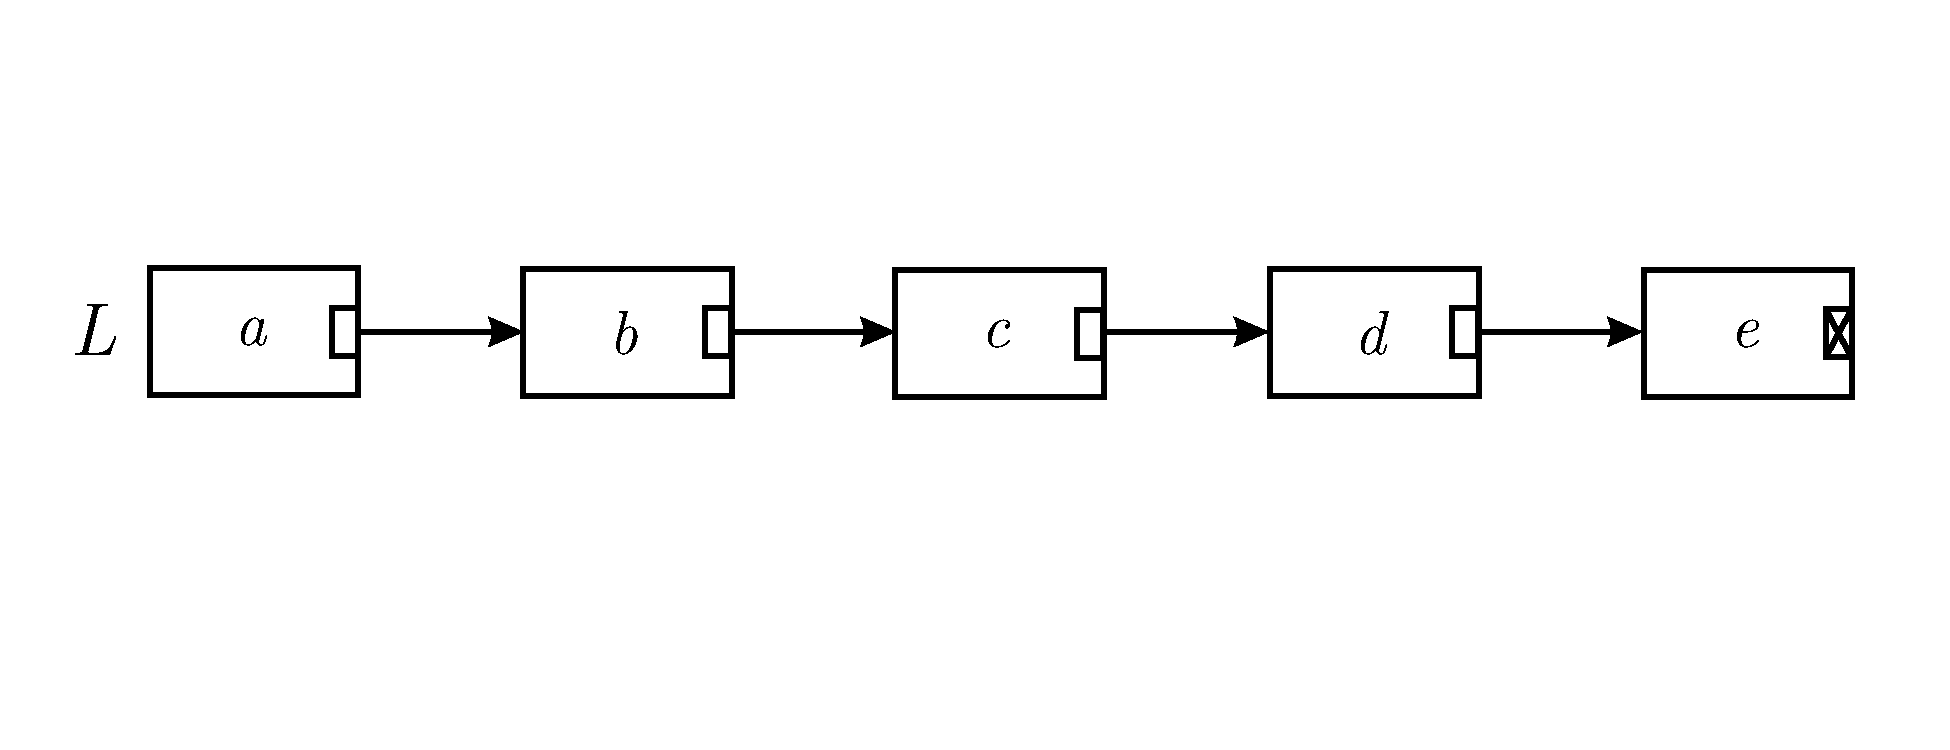
\includegraphics[scale=0.33]{figs/ch3/split_list_input_list.pdf}
\caption{یک لیست پیوندی نمونه به عنوان ورودی تابع {\lr{\textsc{SplitList}}}}\label{ch3:fig:splitListInputList}
\end{center}
\end{figure}

\begin{figure}[H]
\begin{center}
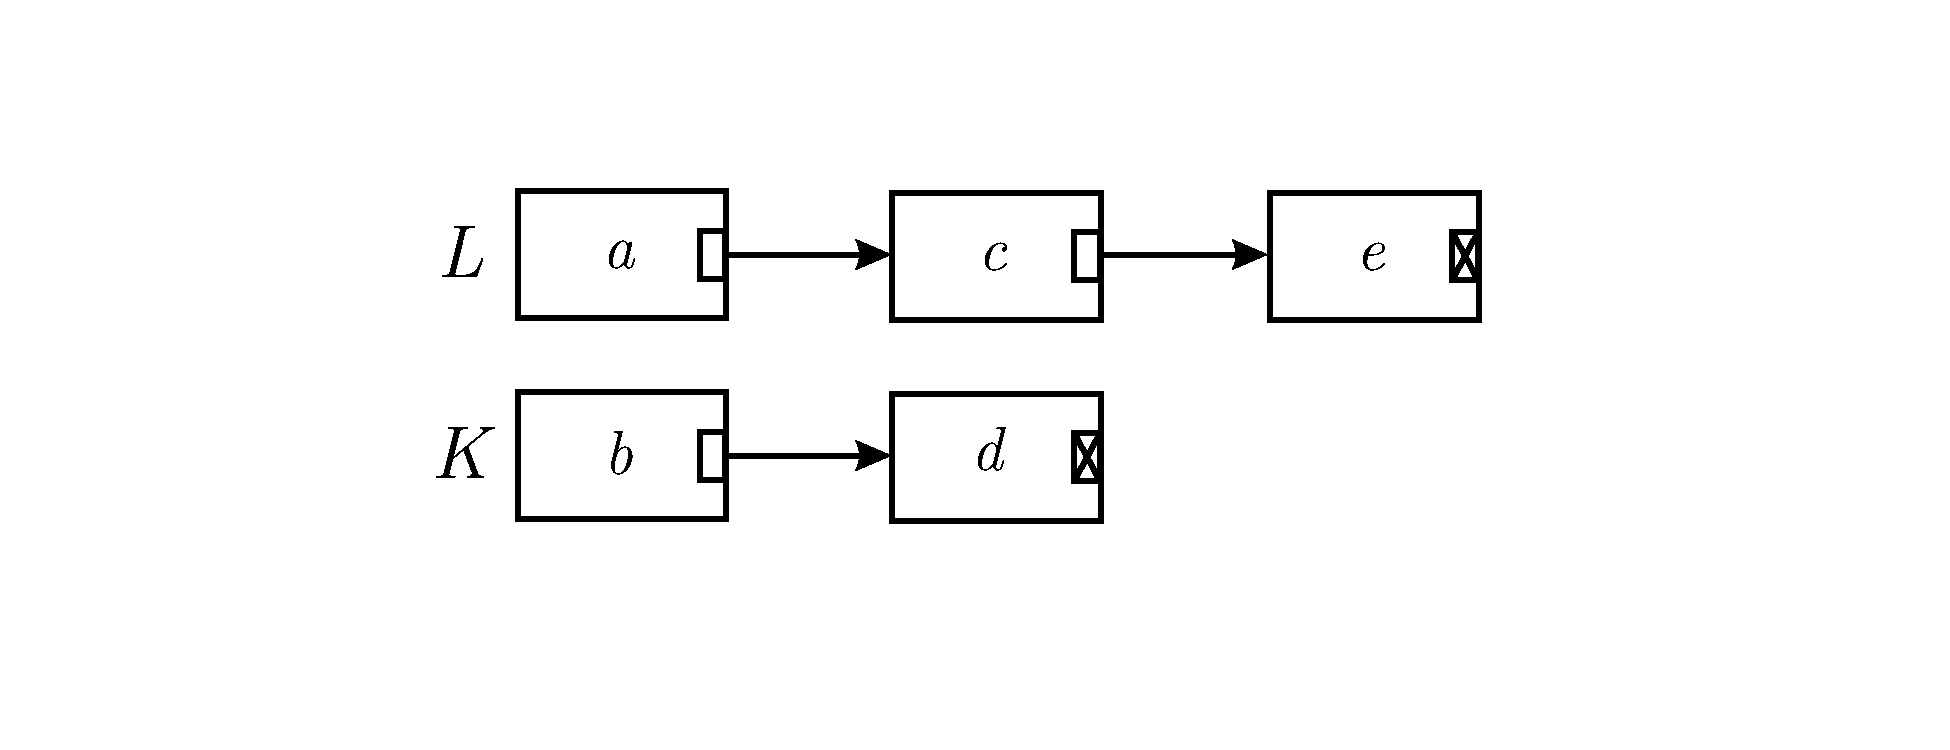
\includegraphics[scale=0.33]{figs/ch3/split_list_output_lists.pdf}
\caption{لیست‌های حاصل از اجرای تابع {\lr{\textsc{SplitList}}}}\label{ch3:fig:splitListOutputLists}
\end{center}
\end{figure}

\پاسخ

شبه کد الگوریتم جداسازی عناصر با شماره‌ی زوج از لیست ورودی در الگوریتم {\eqref{ch3:alg:split}} آمده است.
\begin{algorithm}
\caption{جداسازی عناصر با شماره‌ی زوج یک لیست پیوندی یکطرفه}\label{ch3:alg:split}
\begin{latin}
\begin{algorithmic}[1]
\Function{SplitList}{$L$}
		\If{$L \isequal \const{null} \Or \attrib{L}{next} \isequal \const{null}$}
				\State $K \gets \const{null}$
		\Else
				\State	$K \gets \attrib{L}{next}$
				\State	$\attrib{L}{next} \gets \attribb{L}{next}{next}$
				\State	$\attrib{K}{next} \gets $\bcall{SplitList}{$\attrib{L}{next}$}
		\EndIf
		\State	\Return $K$
\EndFunction
\end{algorithmic}
\end{latin}
\end{algorithm}

اگر لیست {$L$} تهی باشد آنگاه تنها کافیست لیست {$K$} را نیز برابر با تهی قرار دهیم. همچنین هنگامی که لیست {$L$} دارای تنها یک عنصر است  باید لیست {$K$} را برابر با تهی قرار دهیم زیرا در حالتی که فقط یک عنصر وجود دارد این عنصر دارای شماره یک است و در نتیجه لیست {$L$} باید شامل آن عنصر بوده و لیست {$K$} تهی باشد.

اگر لیست {$L$} دارای بیش از یک عنصر باشد آنگاه ابتدا لیست {$K$} به عنصر دوم لیست {$L$} اشاره کرده و سپس عنصر اول لیست {$L$} به عنصر سوم لیست {$L$} اشاره می‌کند. به این ترتیب {$L$} شامل عناصر با شماره‌های {$n ,\ldots , 4,3,1$}  و {$K$} شامل عنصر با شماره‌ی دو خواهد بود. سپس زیربرنامه‌ی {\bcall{SplitList}{}} به صورت بازگشتی  فراخوانی می‌شود تا به همین ترتیب عناصر با شماره‌ی فرد در لیست {$L$} و عناصر با شماره‌ی زوج در لیست {$K$} قرار بگیرند.

\سوال دو لیست پیوندی یکطرفه‌ی {\lr{L1}} و {\lr{L2}} را در نظر بگیرید. مقادیر موجود در این دو لیست به صورت صعودی مرتب هستند. تابعی غیربازگشتی به نام {\bcall{Merge}{}} بنویسید که تمام عناصر دو لیست {\lr{L1}} و {\lr{L2}} را در لیست جدید {\lr{L3}} درج کند به شکلی که عناصر لیست {\lr{L3}} نیز به صورت صعودی مرتب باشند. برای مثال اگر دو لیست نشان داده شده در شکل {\eqref{ch3:fig:mrgBefore}} به عنوان ورودی تابع {\bcall{Merge}{}} داده شوند آنگاه پس از پایان اجرای زیربرنامه باید به لیست جدیدی مانند آنچه در شکل {\eqref{ch3:fig:mrgAfter}} نمایش داده شده است برسیم.

\begin{figure}[H]
\begin{center}
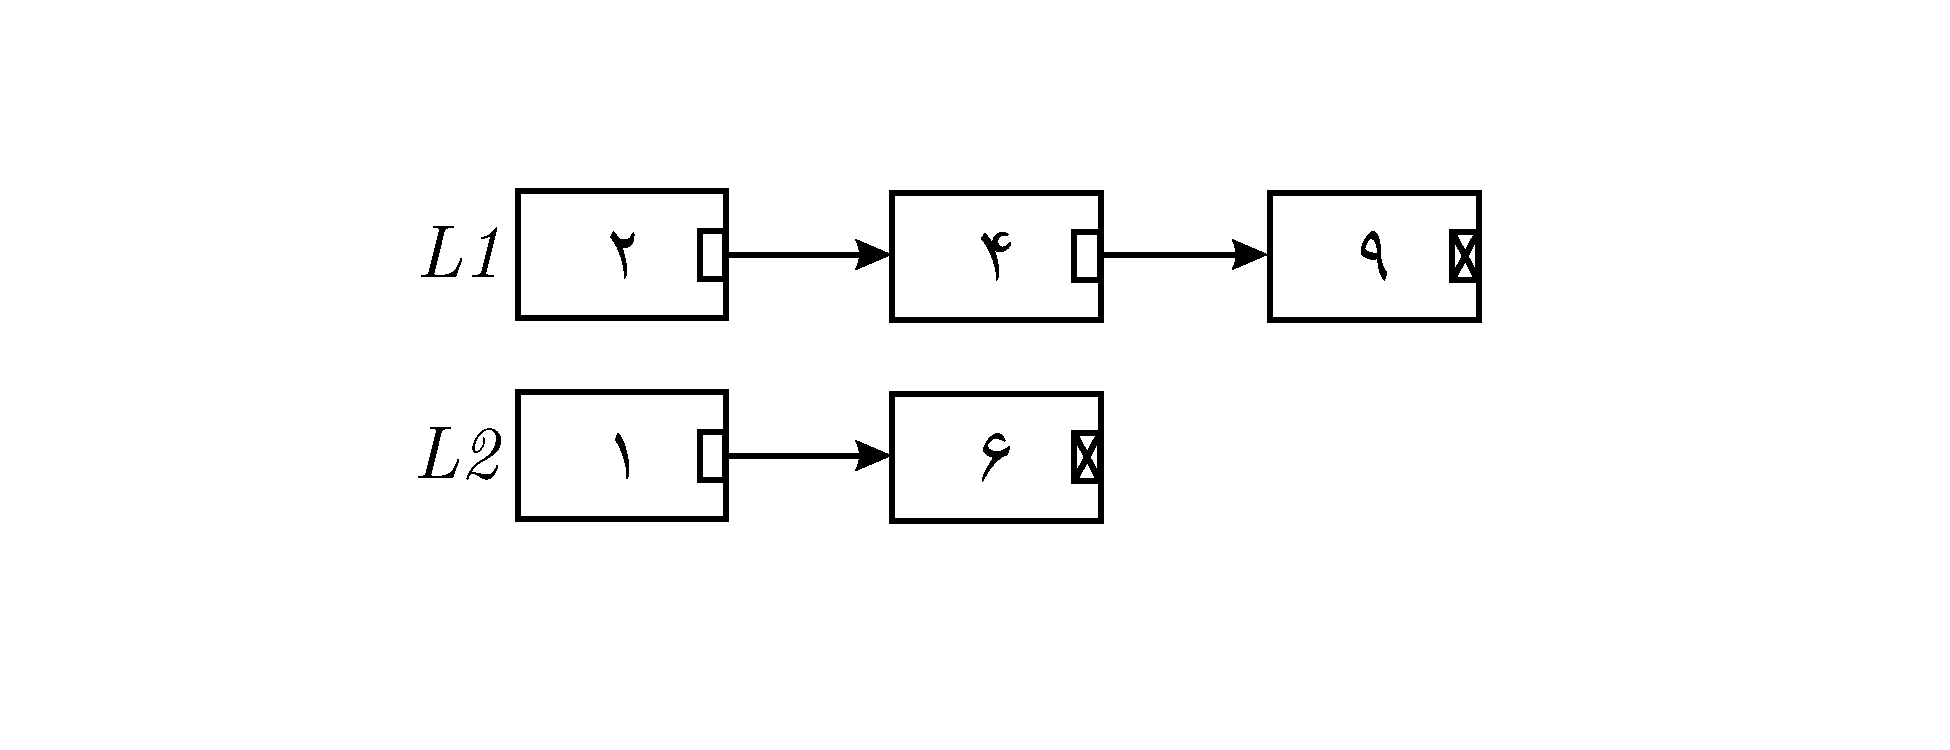
\includegraphics[scale=0.33]{figs/ch3/merge_input_lists.pdf}
\caption{دو لیست پیوندی نمونه به عنوان ورودی تابع {\lr{\textsc{Merge}}}}\label{ch3:fig:mrgBefore}
\end{center}
\end{figure}

\begin{figure}[H]
\begin{center}
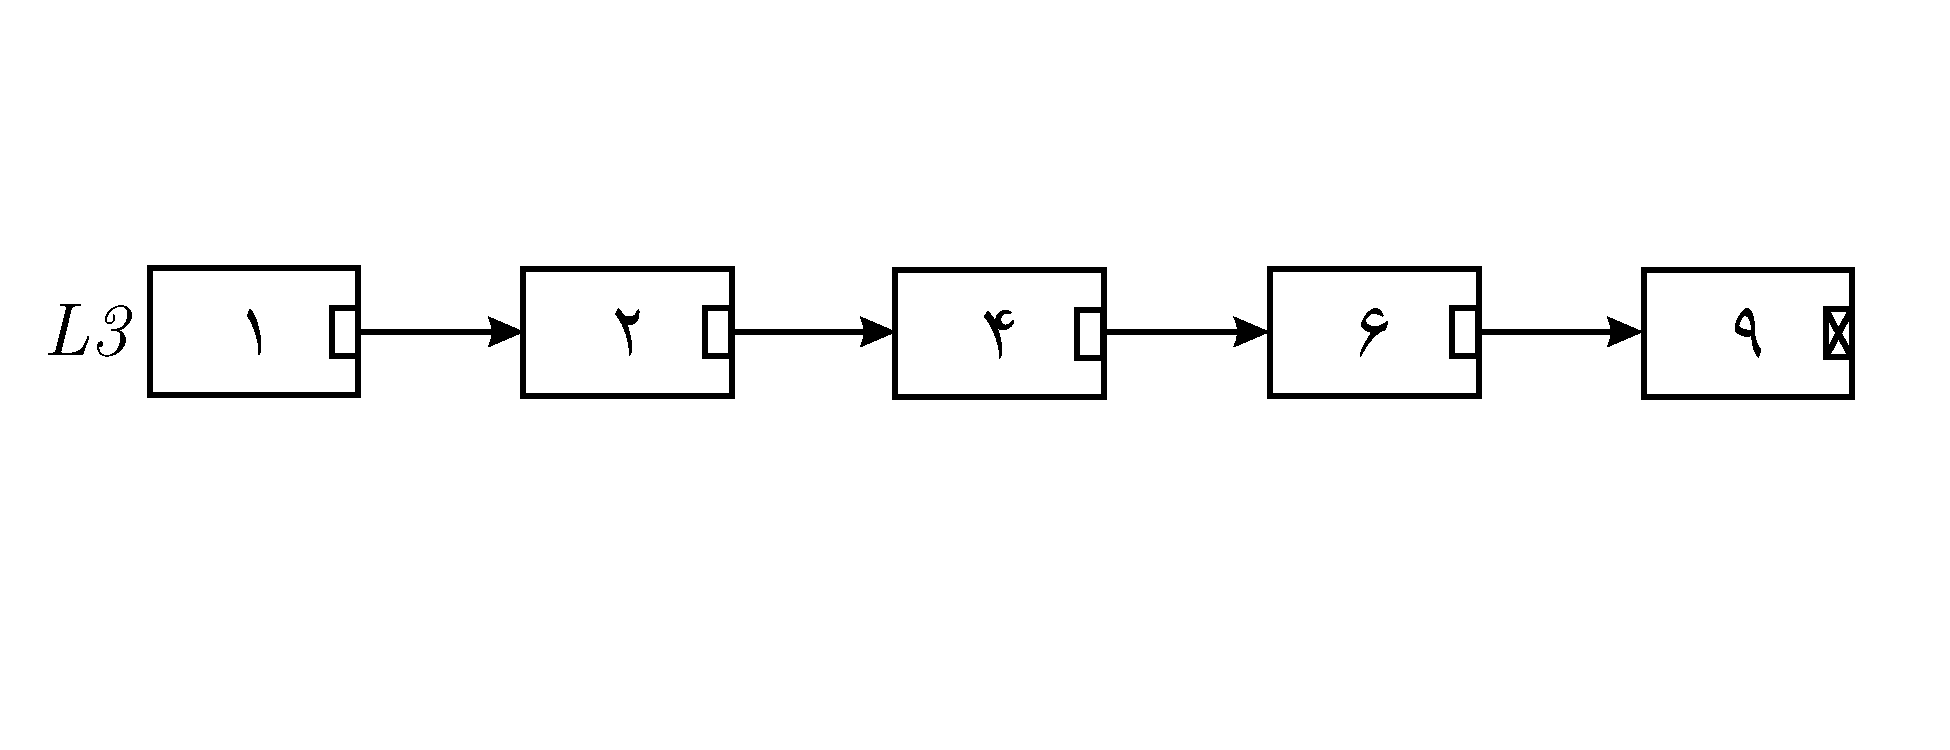
\includegraphics[scale=0.33]{figs/ch3/merge_output_list.pdf}
\caption{%
لیست پیوندی حاصل از اجرای تابع {\lr{\textsc{Merge}}} بر روی لیست‌های پیوندی شکل {\eqref{ch3:fig:mrgBefore}}
}
\label{ch3:fig:mrgAfter}
\end{center}
\end{figure}

\پاسخ

شبه کد تابع ادغام عناصر دو لیست پیوندی یکطرفه در الگوریتم {\eqref{ch3:alg:merge}} آورده شده است. بیان نحوه‌ی عملکرد این تابع در ادامه آمده است. 

\begin{algorithm}[H]
\caption{ادغام عناصر دو لیست پیوندی یکطرفه}\label{ch3:alg:merge}
\begin{latin}
\begin{algorithmic}[1]
\Function{Merge}{$\id{L1},\id{L2}$}
			\State	\bcall{New}{$\id{L3}$}
			\State	$p \gets \id{L3}$
            \algstore{mergeBrk}
\end{algorithmic}
\end{latin}
\end{algorithm}

\begin{algorithm}
\caption*{ادغام عناصر دو لیست پیوندی یکطرفه - ادامه}
\begin{latin}
\begin{algorithmic}[1]
			\algrestore{mergeBrk}
			\State	$q \gets \id{L1}$
			\State	$r \gets \id{L2}$
			\While{$q \neq \const{null} \And r \neq  \const{null}$}\label{ch3:alg:line:mrgWhileBegin}	
					\State	\bcall{New}{$\attrib{p}{next}$}
					\If{$\attrib{q}{data} < \attrib{r}{data}$}
							\State	$\attrib{p}{data} \gets \attrib{q}{data}$
							\State	$q \gets \attrib{q}{next}$
					\Else
							\State	$\attrib{p}{data} \gets \attrib{r}{data}$
							\State	$r \gets \attrib{r}{next}$
					\EndIf
					\State	$p \gets \attrib{p}{next}$
			\EndWhile\ \label{ch3:alg:line:mrgWhileEnd}
			\If{$q \isequal \const{null}$}\label{ch3:alg:line:mrgFirstIfBegin}
					\While{$r \neq \const{null}$}
							\State	$\attrib{p}{data} \gets \attrib{r}{data}$
							\If{$\attrib{r}{next} \neq \const{null}$}
									\State	\bcall{New}{$\attrib{p}{next}$}
									\State	$p \gets \attrib{p}{next}$
							\EndIf
							\State	$r \gets \attrib{r}{next}$
					\EndWhile
			\EndIf\ \label{ch3:alg:line:mrgFirstIfEnd}
			\If{$r \isequal \const{null}$}\label{ch3:alg:line:mrgSecIfBegin}
					\While{$q \neq \const{null}$}
							\State	$\attrib{p}{data} \gets \attrib{q}{data}$
							\If{$\attrib{q}{next} \neq \const{null}$}
									\State	\bcall{New}{$\attrib{p}{next}$}
									\State	$p \gets \attrib{p}{next}$
							\EndIf
							\State	$q \gets \attrib{q}{next}$
					\EndWhile
			\EndIf\ \label{ch3:alg:line:mrgSecIfEnd}
		\State	\Return $\id{L3}$
\EndFunction
\end{algorithmic}
\end{latin}
\end{algorithm}

حلقه‌ی {\lr{while}} موجود در خطوط {\ref{ch3:alg:line:mrgWhileBegin}} تا {\ref{ch3:alg:line:mrgWhileEnd}} در هر دور از اجرای خود از میان دو عنصر جاری لیست‌های {\lr{L1}} و {\lr{L2}}، عنصری را که دارای مقدار کمتری است انتخاب کرده و در لیست {\lr{L3}} درج می‌کند. این حلقه زمانی پایان می‌یابد که حداقل یکی از دو لیست {\lr{L1}} یا {\lr{L2}} به انتهای خود برسند. پس از پایان اجرای حلقه باید بررسی شود که کدام لیست به انتهای خود رسیده است تا بتوان عناصر باقیمانده در لیست دیگر را در انتهای لیست {\lr{L3}} درج کرد. اگر لیست {\lr{L1}} به انتهای خود رسیده باشد باید عناصر باقیمانده در لیست {\lr{L2}} را به لیست {\lr{L3}} اضافه کرد (خطوط {\ref{ch3:alg:line:mrgFirstIfBegin}} تا {\ref{ch3:alg:line:mrgFirstIfEnd}}) و اگر لیست {\lr{L2}} به انتهای خود رسیده باشد آنگاه عناصر باقیمانده در لیست {\lr{L1}} باید در لیست {\lr{L3}} درج شوند (خطوط {\ref{ch3:alg:line:mrgSecIfBegin}} تا {\ref{ch3:alg:line:mrgSecIfEnd}}).

\سوال زیربرنامه‌ای غیربازگشتی بنویسید که عناصری از یک لیست پیوندی یکطرفه که دارای مقدار تکراری هستند را از لیست حذف کند. برای مثال اگر ورودی زیربرنامه لیست {$L=\langle a,b,a,c,b,d,d\rangle$} باشد آنگاه خروجی زیربرنامه باید لیست {$L=\langle a,b,c,d\rangle$} باشد. نسخه بازگشتی چنین زیربرنامه‌ای  را نیز طراحی کنید.

\پاسخ

شبه کد نسخه‌ی غیربازگشتی زیربرنامه‌ی حذف مقادیر تکراری یک لیست پیوندی یکطرفه در قالب الگوریتم {\eqref{ch3:alg:rmvRedun}} نمایش داده شده است.
\begin{algorithm}
\caption{حذف عناصر با مقادیر تکراری از یک لیست پیوندی یکطرفه}\label{ch3:alg:rmvRedun}
\begin{latin}
\begin{algorithmic}[1]
\Procedure{RemoveRedundant}{$L$}
		\If{$L \isequal \const{null}$}
				\State	\Return
		\EndIf
		\State	$p \gets L$
		\While{$\attrib{p}{next} \neq \const{null}$}
				\State	$q \gets p$
				\While{$\attrib{q}{next} \neq \const{null}$}
						\If{$\attribb{q}{next}{data} \isequal \attrib{p}{data}$}
								\State	$r \gets \attrib{q}{next}$
								\State	$\attrib{q}{next} \gets \attrib{r}{next}$
								\State	\bcall{Free}{$r$}
						\Else
								\State	$q \gets \attrib{q}{next}$
						\EndIf
				\EndWhile
				\State	$p \gets \attrib{p}{next}$
		\EndWhile		
\EndProcedure
\end{algorithmic}
\end{latin}
\end{algorithm}

روش عملکرد زیربرنامه‌ی {\bcall{RemoveRedundant}{}} به این صورت است که در هر بار اجرای حلقه‌ی {\lr{while}} بیرونی، یک عنصر از لیست {$L$} که {$p$} به آن اشاره دارد به عنوان عنصر جاری در نظر گرفته می‌شود و عمل پیمایش در لیست {$L$}، از عنصر جاری به بعد، آغاز می‌شود. در حین انجام پیمایش اگر عنصری یافت شود که مقدار آن برابر با مقدار عنصر جاری باشد آنگاه این عنصر از لیست حذف می‌شود. اجرای حلقه‌ی {\lr{while}} بیرونی زمانی متوقف می‌شود که به ازای تمام عناصر لیست {$L$} عمل پیمایش انجام شده و تمام عناصر با مقادیر تکراری حذف شده باشند.

نسخه‌ی بازگشتی زیربرنامه‌ی حذف مقادیر تکراری یک لیست پیوندی یکطرفه در الگوریتم {\eqref{ch3:alg:recRmvRedun}} آمده است. نسخه‌ی بازگشتی به این صورت عمل می‌کند که فرض می‌شود عنصر ابتدایی لیست وجود ندارد و زیربرنامه به صورت بازگشتی با شروع از عنصر دوم لیست ورودی فراخوانی می‌شود. پس از بازگشت از فراخوانی خط {\ref{ch3:alg:line:recCall}}، دارای لیستی خواهیم بود که ممکن است تعدادی از عناصر آن دارای مقدار یکسان با مقدار عنصر اول لیست باشند. به این ترتیب با شروع از ابتدای لیست و با انجام عمل پیمایش، هر عنصری که دارای مقدار یکسان با مقدار عنصر اول بود از لیست حذف می‌شود.
\begin{algorithm}
\caption{حذف عناصر با مقادیر تکراری از یک لیست پیوندی یکطرفه به صورت بازگشتی}\label{ch3:alg:recRmvRedun}
\begin{latin}
\begin{algorithmic}[1]
\Procedure{RemoveRedundant}{$L$}
		\If{$L \isequal \const{null} \Or \attrib{L}{next} \isequal \const{null}$}				
				\State	\Return
		\EndIf
		\State	\bcall{RemoveRedundant}{$\attrib{L}{next}$}\label{ch3:alg:line:recCall}
		\State	$p \gets L$
		\While{$\attrib{p}{next} \neq \const {null}$}
				\If{$\attribb{p}{next}{data} \isequal \attrib{L}{data}$}
						\State	$r \gets \attrib{p}{next}$
						\State	$\attrib{p}{next} \gets \attrib{r}{next}$
						\State	\bcall{Free}{$r$}
				\Else
						\State	$p \gets \attrib{p}{next}$
				\EndIf
		\EndWhile			
\EndProcedure
\end{algorithmic}
\end{latin}
\end{algorithm}

\سوال فرض کنید دارای یک لیست پیوندی یکطرفه به نام {$L$} و اشاره‌گر {$p$} هستیم. {$p$} به یکی از عناصر لیست {$L$} که عنصر آخر لیست نیست اشاره دارد. به جز {$p$} هیچ اشاره‌گر دیگری به هیچ یک از عناصر لیست {$L$} وجود ندارد مگر اینکه از ابتدای لیست پیمایش انجام شود. قطعه کدی از مرتبه‌ی {$O(1)$} بنویسید که مقدار موجود در عنصری که {$p$} به آن اشاره دارد را از لیست {$L$} حذف کند.

\پاسخ

قطعه کد لازم برای حذف مقدار مورد نظر در ادامه آمده است.
\begin{latin}
\begin{algorithmic}[1]
		\State	$\attrib{p}{data} \gets \attribb{p}{next}{data}$
		\State	$t \gets \attrib{p}{next}$
		\State	$\attrib{p}{next} \gets \attribb{p}{next}{next}$
		\State	\bcall{Free}{$t$}
\end{algorithmic}
\end{latin}

\سوال دو عدد صحیح مثبت را در نظر بگیرید که دارای تعداد ارقام یکسان هستند. هر عدد در یک لیست پیوندی یکطرفه ذخیره شده‌ است. روش ذخیره‌سازی عدد در لیست پیوندی یکطرفه به این صورت است که رقم یکان در گره‌ی ابتدای لیست، رقم دهگان در گره‌ی دوم، رقم صدگان در گره‌ی سوم و به همین ترتیب تا رقم آخر که در گره‌ی انتهایی لیست قرار می‌گیرد. تابعی بنویسید که دو عدد صحیح، در قالب مطرح شده، را به عنوان ورودی دریافت کرده و یک لیست پیوندی یکطرفه که حاوی حاصل جمع دو عدد ورودی است را به عنوان خروجی بازگرداند.

\پاسخ

شبه کد خواسته شده در قالب الگوریتم {\eqref{ch3:alg:add}} نشان داده شده است. در این الگوریتم {$M$} اشاره‌گر به ابتدای لیست پیوندی حاوی عدد اول و {$N$} اشاره‌گر به ابتدای لیست پیوندی حاوی عدد دوم است. در ادامه به روش کار الگوریتم اشاره خواهد شد.

\begin{algorithm}[H]
\caption{جمع دو عدد صحیح مثبت که در قالب لیست‌های پیوندی یکطرفه داده شده‌اند}\label{ch3:alg:add}
\begin{latin}
\begin{algorithmic}[1]
\Function{Add}{$M,N$}
		\If{$M \isequal \const{null} \And N \isequal \const{null}$}	
				\State	\Return \const{null}
		\EndIf
		\State \bcall{New}{$L$}
		\State $p \gets M$
		\State $q \gets N$
		\State $r \gets L$
		\State $\id{carry} \gets 0$
		\While{$p \neq \const{null}$}
			\State $\id{sum} \gets \attrib{p}{data} + \attrib{q}{data} + \id{carry}$
			\State $\id{carry} \gets \id{sum} \div 10$
			\State $\id{sum} \gets \id{sum} \bmod 10$
			\State $\attrib{r}{data} \gets \id{sum}$
			\State $\attrib{r}{next} \gets \const{null}$
			\State $p \gets \attrib{p}{next}$
			\State $q \gets \attrib{q}{next}$
			\If{$p \neq \const{null}$}
				\State \bcall{New}{\attrib{r}{next}}
		\algstore{addBrk}
\end{algorithmic}
\end{latin}
\end{algorithm}

\begin{algorithm}
\caption*{جمع دو عدد صحیح مثبت که در قالب لیست‌های پیوندی یکطرفه داده شده‌اند - ادامه}
\begin{latin}
\begin{algorithmic}[1]
			\algrestore{addBrk}
				\State $r \gets \attrib{r}{next}$
				\State $\attrib{r}{next} \gets \const{null}$
			\EndIf
		\EndWhile
		\If{$\id{carry} \neq 0$}
			\State \bcall{New}{\attrib{r}{next}}	
			\State $r \gets \attrib{r}{next}$
			\State $\attrib{r}{data} \gets \id{carry}$
			\State $\attrib{r}{next} \gets \const{null}$
		\EndIf
		\State \Return $L$
\EndFunction
\end{algorithmic}
\end{latin}
\end{algorithm}

با توجه به اینکه در صورت سوال بیان شده است که دو عدد ورودی دارای تعداد ارقام یکسان هستند در نتیجه می‌توان دو حالت را برای لیست‌های پیوندی ورودی در نظر گرفت:
\شروع{فقرات}
\فقره هر دو لیست تهی هستند،
\فقره هر دو لیست غیر تهی و دارای تعداد گره‌های یکسان هستند.
\پایان{فقرات}
در حالت اول، یعنی تهی بودن هر دو لیست، کاری برای انجام دادن وجود ندارد و تنها مقدار {\const{null}} به عنوان خروجی الگوریتم برگشت داده می‌شود.

در حالت دوم به کمک یک حلقه شروع به پیمایش هر دو لیست می‌کنیم تا ارقام دو عدد را با یکدیگر جمع کنیم. شرط حلقه‌ به جای
{\lr{$p \neq$ \const{null}}} می‌توانست {\lr{$q \neq$ \const{null}}} هم باشد زیرا هر دو لیست دارای طول یکسان هستند. در هر دور از اجرای حلقه دو رقم جاری با یکدیگر جمع می‌شوند تا یک مقدار به عنوان حاصل جمع (متغیر {\id{sum}}) و مقدار دیگر به عنوان رقم نقلی (متغیر {\id{carry}}) به دست بیایند. مقدار متغیر {\id{sum}} در فیلد داده‌‌ای گره‌ی جاری لیست حاوی حاصل جمع قرار می‌گیرد و مقدار {\id{carry}} در دور بعدی اجرای حلقه به حاصل جمع دو رقم بعدی اضافه می‌شود.

پس از پایان اجرای حلقه باید بررسی کرد که آیا رقم نقلی صفر است یا خیر. اگر رقم نقلی صفر باشد کار خاصی انجام نمی‌شود در غیر این صورت باید رقم نقلی را به عنوان با ارزشترین رقم به حاصل جمع دو عدد اضافه کرد. برای این منظور یک گره در انتهای لیست پیوندی حاوی حاصل جمع ایجاد شده و مقدار متغیر {\id{carry}} در فیلد داده‌ای آن قرار می‌گیرد.

در انتهای اجرای الگوریتم اشاره‌گر به ابتدای لیست پیوندی حاوی حاصل جمع دو عدد ورودی به عنوان خروجی الگوریتم بازگردانده می‌شود.

\قسمت{لیست‌ پیوندی دوطرفه}

\سوال لیست پیوندی دوطرفه {$L$} را در نظر بگیرید. گره‌ای مانند {$n$} در {$L$} دارای دو اشاره‌گر است که یکی به گره‌ی قبلی و دیگری به گره‌ی بعدی اشاره دارد (اشاره‌گرهای {\id{prev}} و {\id{next}}). با ترفندی خاص می‌توان لیست پیوندی دوطرفه {$L'$} را تنها با یک اشاره‌گر به ازای هر گره پیاده‌سازی کرد که در این صورت فضای مصرفی به ازای هر گره در یک لیست پیوندی دوطرفه برابر با فضای مصرفی گره‌ای در یک لیست پیوندی یکطرفه خواهد بود. این ترفند به این صورت است که هر گره مانند {$n'$} در {$L'$} دارای اشاره‌گری به نام {\id{pn}} است. فرض کنید مقدار هر اشاره‌گر را بتوان به عنوان عددی {$k$} بیتی تفسیر کرد. به ازای هر گره مانند {$n$} در {$L$} گره‌ای مانند {$n'$} در {$L'$} در نظر می‌گیریم و قرار می‌دهیم {\lr{\attrib{n'}{pn} $=$ \attrib{n}{\id{prev}} $\oplus$ \attrib{n}{\id{next}}}
و  {\lr{\attrib{n'}{\id{data}} $=$ \attrib{n}{\id{data}}}} (نماد {$\oplus$} نشان‌دهنده عملگر یای-انحصاری\پانویس{\lr{Exclusive-Or (XOR)}}} است). از لیست {$L'$} با عنوان لیست پیوندی یای-انحصاری\پانویس{{\lr{Xor linked list}}} یاد می‌شود.

با توجه به توضیحات داده شده الگوریتمی بنویسید که لیستی از نوع {$L'$}، مقدار {$x$} و اشاره‌گر {$p$} را دریافت کرده و گره‌ای با مقدار {$x$} را بعد از گره‌ای که {$p$} به آن اشاره دارد درج کند. اگر  {$p$} دارای مقدار {\const{null}} باشد بدین معنی است که گره‌ی جدید باید به عنوان گره ابتدایی لیست درج شود. (مقدار {\const{Null}} را هنگام تفسیر به صورت عددی، معادل با صفر در نظر بگیرید).

\پاسخ

\begin{figure}
\begin{center}
\subfloat[یک لیست پیوندی دوطرفه]{%
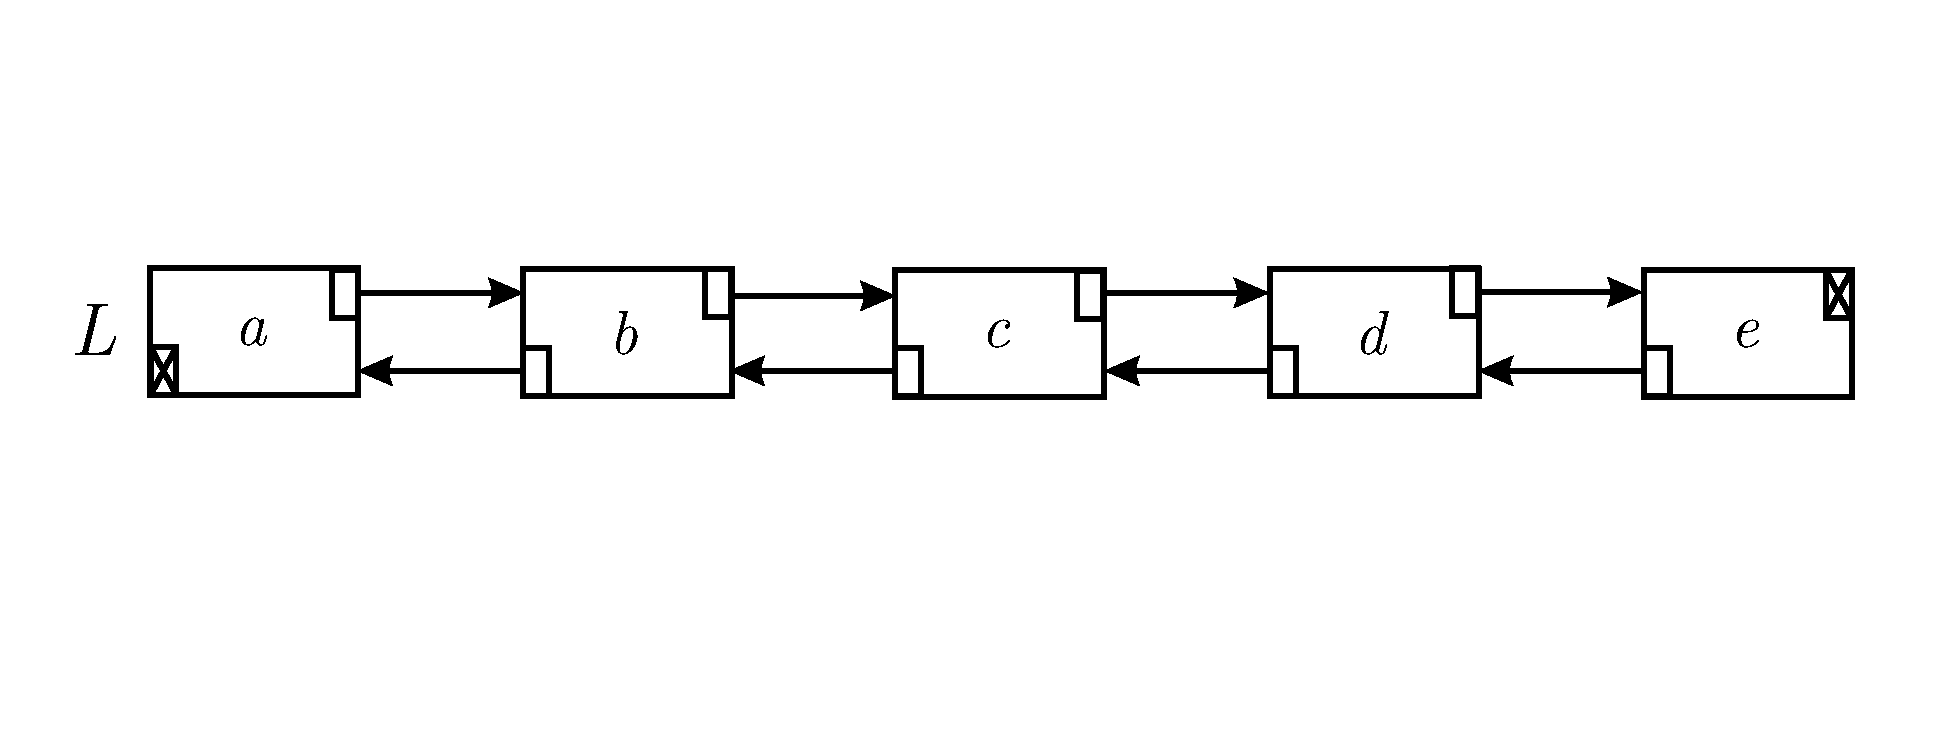
\includegraphics[scale=0.33]{figs/ch3/doubly_linked_list.pdf}\label{ch3:fig:dblLnkLst}
}\\[0.7cm]
\subfloat[لیست پیوندی یای-انحصاری معادل با لیست پیوندی قسمت (آ)]{%
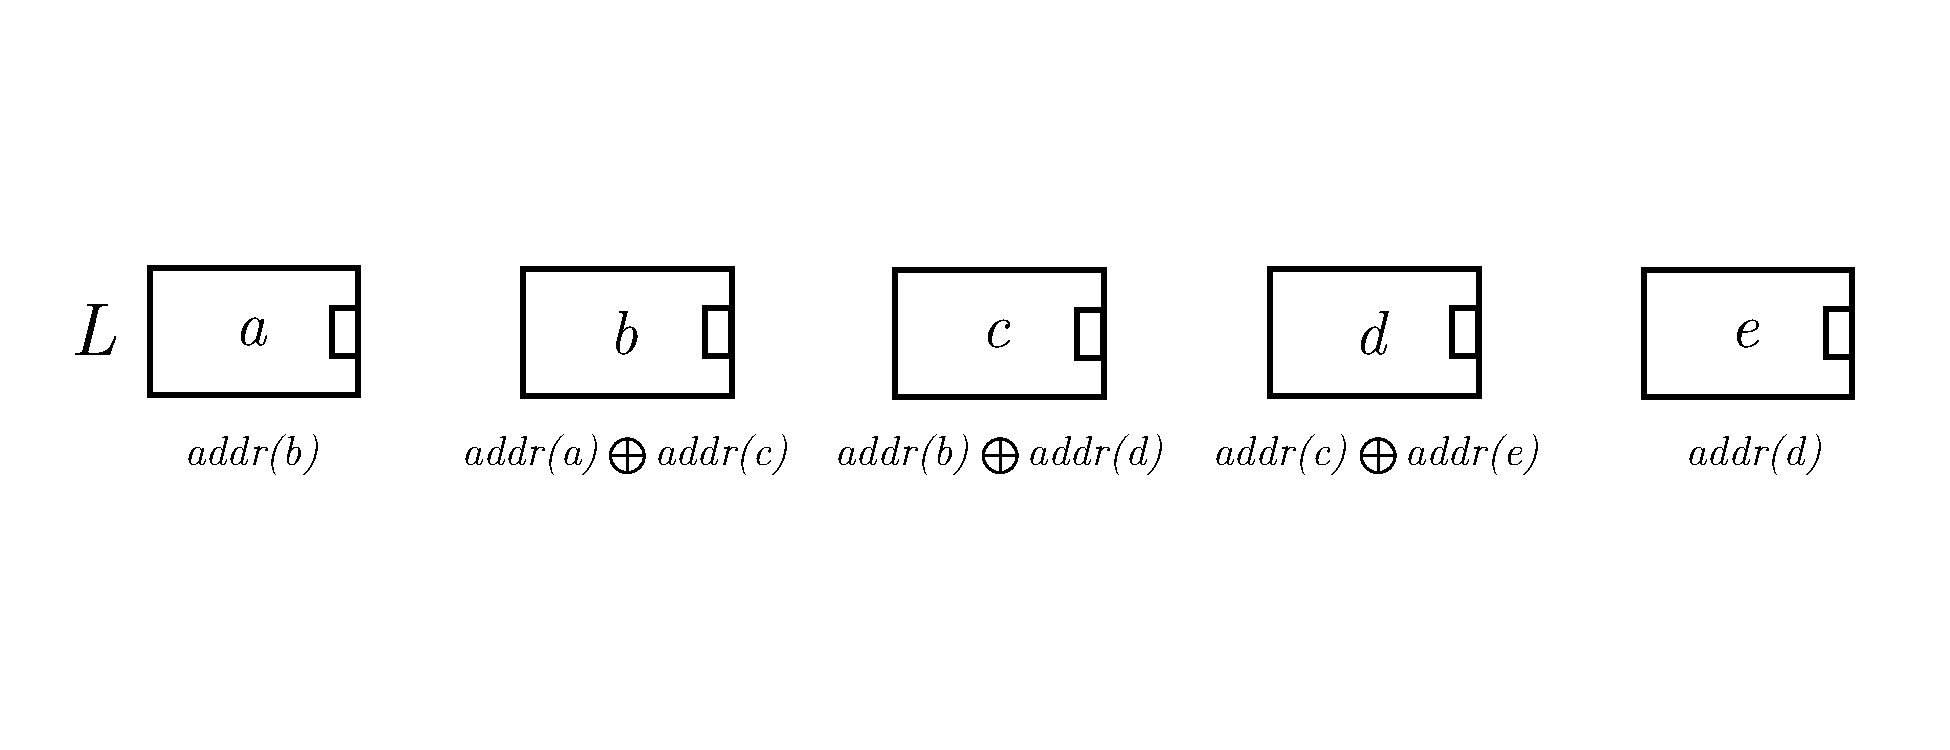
\includegraphics[scale=0.33]{figs/ch3/xor_linked_list.pdf}\label{ch3:fig:xorLnkLst}
}
\caption{یک لیست پیوندی دوطرفه و لیست پیوندی یای-انحصاری معادل آن.}\label{ch3:fig:dblXorLnkLst}
\end{center}
\end{figure}

شکل {\eqref{ch3:fig:dblXorLnkLst}} نشان‌دهنده‌ی یک لیست پیوندی دوطرفه و لیست پیوندی یای-انحصاری معادل با آن است. در شکل {\eqref{ch3:fig:xorLnkLst}} مقدار اشاره‌گر {\id{pn}} هر گره در زیر آن نوشته شده است. برای مثال مقدار اشاره‌گر {\id{np}} برای گره‌ای با مقدار داده‌ای {$a$} برابر با {\lr{\const{null} $\oplus\ \mathit{addr}(b)$}} است و این یعنی آدرس گره‌ی قبلی {$a$} (که برابر است با {\const{null}}) با آدرس گره‌ی بعدی {$a$} (که برابر است با {$\mathit{addr}(b)$}) با یکدیگر یای-انحصاری شده‌اند. چون می‌دانیم حاصل یای انحصاری هر مقداری با صفر برابر با خود همان مقدار است و از طرفی ثابت {\const{null}} را برابر با عدد صفر در نظر گرفتیم پس در نهایت مقدار اشاره‌گر {\id{pn}} گره {$a$} برابر است با {$\mathit{addr}(b)$}.

برای نوشتن الگوریتم درج مقداری جدید در یک لیست پیوندی یای-انحصاری باید به دو مورد زیر توجه کرد:
 \شروع{فقرات}
\فقره برای درج مقداری جدید در یک لیست پیوندی (چه یکطرفه و چه دوطرفه) باید دو حالت زیر را از یکدیگر جدا کرد:
\شروع{فقرات}
\فقره مقدار جدید در ابتدای لیست درج شود، 
\فقره مقدار جدید در جایی به جز ابتدای لیست درج شود. 
\پایان{فقرات}
\فقره برای پیمایش یک لیست پیوندی یای-انحصاری نمی‌توان با عبارتی همچون {$q\gets \attrib{q}{pn}$} به گره‌ی بعدی یا قبلی در لیست رفت.
\پایان{فقرات}

از الگوریتم {\eqref{ch3:alg:insXorLnkLst}} می‌توان برای درج عنصری جدید در یک لیست پیوندی یای-انحصاری استفاده کرد.

\begin{algorithm}[H]
\caption{درج عنصری جدید در یک لیست پیوندی یای-انحصاری}\label{ch3:alg:insXorLnkLst}
\begin{latin}
\begin{algorithmic}[1]
\Procedure{Insert}{$L,x,p$}
    \State    \bcall{New}{$n$}
    \State    $\attrib{n}{data} \gets x$
    \If{$p \isequal \const{null}$}
        \State    $\attrib{n}{pn} \gets L$\label{ch3:alg:ln:xorLnkLst1caseBgn}
        \State    $\attrib{L}{pn} \gets n \oplus \attrib{L}{pn}$
        \State    $L \gets n$\label{ch3:alg:ln:xorLnkLst1caseEnd}
    \Else
        \State    $q \gets \const{null}$\label{ch3:alg:ln:xorLnkLst2caseBgn}
        \State    $r \gets L$
        \While{$r \neq p$}
            \State    $q \gets r$
            \State    $r \gets q \oplus \attrib{r}{pn}$
        \EndWhile
        \State    $\id{prev} \gets r$\label{ch3:alg:ln:ptrsInitBgn}
        \State    $\id{next} \gets \attrib{r}{pn} \oplus q$
        \State    $\attrib{n}{pn} \gets \id{prev} \oplus \id{next}$
        \State    $\attrib{r}{pn} \gets q \oplus n$
        \If{$\id{next}\neq$ \const{null}}
            \State    $\attrib{next}{pn} \gets n \oplus r \oplus \attrib{next}{pn}$
        \EndIf\label{ch3:alg:ln:ptrsInitEnd}
        \label{ch3:alg:ln:xorLnkLst2caseEnd}
    \EndIf
\EndProcedure
\end{algorithmic}
\end{latin}
\end{algorithm}

خطوط {\ref{ch3:alg:ln:xorLnkLst1caseBgn}} تا {\ref{ch3:alg:ln:xorLnkLst1caseEnd}} نشان‌دهنده‌ی حالتی است که عنصر جدید باید در ابتدای لیست درج شود. در گام اول باید اشاره‌گر گره‌ی {$n$} مقداردهی شود. مقدار اشاره‌گر گره‌ی {$n$} باید برابر با یای-انحصاری آدرس گره‌ی قبلی و آدرس گره‌ی بعدی {$n$} باشد که با در نظر گرفتن شکل {\eqref{ch3:fig:xorLnkLst}} خواهیم داشت {\lr{$\attrib{n}{pn}\gets$\const{null}$\oplus\mathit{addr}(a)$}}. از آنجایی که مقدار ثابت {\const{null}} را برابر با صفر در نظر گرفته‌ایم و همچنین می‌دانیم برای هر عدد {$k$} بیتی مانند {$w$} رابطه {$w\oplus 0=w$} برقرار است در نتیجه داریم {$\attrib{n}{pn}\gets \mathit{addr}(a)$}. چون {$L$} حاوی آدرس گره‌ی {$a$} است در نهایت مقدار اشاره‌گر گره‌ی {$n$} برابر با {$L$} قرار داده شده است. 

در گام دوم باید اشاره‌گر گره‌ی {$a$} (که {$L$} به آن اشاره دارد) مقداردهی شود. آدرس گره‌ی قبلی {$a$} برابر با {$n$} و آدرس گره‌ی بعدی آن برابر با {$\mathit{addr}(b)$} است پس خواهیم داشت {$\attrib{L}{pn}= n\oplus \mathit{addr}(b)$}. چون {$\attrib{L}{pn}$} برابر با {$\mathit{addr}(b)$} است در نهایت مقدار اشاره‌گر گره‌ی {$a$} برابر با {$n\oplus \attrib{L}{pn}$} خواهد شد.

در گام نهایی قرار می‌دهیم {$L\gets n$} تا اشاره‌گر {$L$} به ابتدای لیست اشاره کند زیرا گره‌ی جدید در ابتدای لیست درج شده است و {$L$} باید همواره به گره‌ی ابتدایی لیست اشاره کند.

خطوط {\ref{ch3:alg:ln:xorLnkLst2caseBgn}} تا {\ref{ch3:alg:ln:xorLnkLst2caseEnd}} مربوط به حالتی است که عنصر جدید باید در جایی به جز ابتدای لیست درج شود. در گام اول باید لیست را پیمایش کنیم تا به گره‌ای برسیم که اشاره‌گر {$p$} به آن اشاره دارد. برای رفتن به گره‌ی بعدی از عبارت {$r \gets q \oplus \attrib{r}{pn}$} استفاده شده است. شکل {\eqref{ch3:fig:xorLnkLst}} را در نظر بگیرید و فرض کنید در ابتدای یکی از تکرارهای حلقه، اشاره‌گر {$r$} به گره‌ی {$c$} و اشاره‌گر {$q$} به گره‌ی {$b$} اشاره دارد. چون {$q$} برابر با {$\mathit{addr}(b)$} و {$\attrib{r}{pn}$} برابر با {$\mathit{addr}(b)\oplus \mathit{addr}(d)$} است خواهیم داشت
 {$r\gets\mathit{addr}(b)\oplus\mathit{addr}(b)\oplus\mathit{addr}(d)$}. از آنجایی که برای هر عدد {$k$} بیتی مانند {$w$} داریم {$w\oplus w=0$} پس می‌توان نتیجه گرفت {$r\gets 0\oplus \mathit{addr}(d)$} و این یعنی {$r\gets \mathit{addr}(d)$}. به این ترتیب توانستیم از گره‌ی {$c$} به گره‌ی {$d$} حرکت کنیم. روند پیمایش در لیست به همین ترتیب ادامه می‌یابد تا به گره‌ای برسیم که {$p$} به آن اشاره دارد. پس از پایان اجرای حلقه، اشاره‌گر {$r$} به گره‌ای اشاره دارد که {$p$} نیز به آن اشاره دارد و اشاره‌گر {$q$} به گره‌ی قبلی {$r$} اشاره دارد.

پس از رسیدن به مکان مورد نظر در لیست باید حداکثر سه اشاره‌گر مقداردهی شوند تا گره‌ی جدید در مکان درست خود درج شود. اشاره‌گر اول مربوط به گره‌ی جدید است، اشاره‌گر دوم مربوط به گره‌ای است که باید قبل از گره‌ی جدید قرار بگیرد و اشاره‌گر سوم مربوط به گره‌ای است که باید بعد از گره‌ی جدید قرار بگیرد. زمانی که گره‌ی جدید به عنوان گره‌ی آخر لیست درج می‌شود بدیهی است که اشاره‌گر سومی وجود ندارد و تنها باید دو اشاره‌گر مقداردهی شوند. در خطوط {\ref{ch3:alg:ln:ptrsInitBgn}} تا {\ref{ch3:alg:ln:ptrsInitEnd}} از دو خاصیت عملگر یای-انحصاری، که در پاراگراف‌های قبلی بیان شدند، استفاده شده است تا به اشاره‌گر‌ها مقداردهی شود. برای درک چگونگی عملکرد این خطوط، شکل {\eqref{ch3:fig:xorLnkLst}} را در نظر بگیرید و اجرای این خطوط را بر روی آن دنبال کنید.

\سوال لیست پیوندی دوطرفه‌ی حلقوی {$L$} که غیر تهی و دارای فرد گره است را در نظر بگیرید. تابعی بنویسید که لیست {$L$} را به عنوان ورودی دریافت کرده و اشاره‌گر به گره‌ی وسط {$L$} را به عنوان خروجی برگرداند (توجه: برای به دست آوردن گره‌ی وسط، مجاز به شمارش تعداد گره‌ها نیستید). 

\پاسخ

الگوریتم {\eqref{ch3:alg:findMiddle}} شبه کد یافتن گره وسط در یک لیست پیوندی دوطرفه‌ی حلقوی را نشان می‌دهد. روش کار الگوریتم بسیار ساده است. با استفاده از اشاره‌گر {$p$} از ابتدای لیست شروع کرده و به سمت انتهای لیست حرکت می‌کنیم و با اشاره‌گر {$q$} از انتهای لیست شروع کرده و به سمت ابتدای لیست حرکت می‌کنیم. حرکت از ابتدا به انتها و از انتها به ابتدا تا زمانی ادامه می‌یابد که دو اشاره {$p$} و {$q$} به هم برسند که در این صورت گره‌ای که این دو اشاره‌گر به آن اشاره می‌کنند همان گره وسط لیست خواهد بود. در نهایت اشاره‌گر {$p$} به عنوان اشاره‌گر به گره وسط توسط تابع به عنوان خروجی برگردانده می‌شود (مقدار {$q$} نیز می‌توانست برگردانده شود چون در انتهای اجرای الگوریتم هر دو اشاره‌گر به گره وسط اشاره می‌کنند).

\begin{algorithm}
\caption{یافتن گره وسط در یک لیست پیوندی دوطرفه‌ی حلقوی}\label{ch3:alg:findMiddle}
\begin{latin}
\begin{algorithmic}[1]
\Function{FindMiddle}{$L$}
    \State    $p \gets L$
    \State    $q \gets \attrib{L}{prev}$
    \While{$p \neq q$}
        \State    $p \gets \attrib{p}{next}$
        \State    $q \gets \attrib{q}{prev}$
    \EndWhile
    \State    \Return $p$
\EndFunction
\end{algorithmic}
\end{latin}
\end{algorithm}

\قسمت{لیست‌ اندیسی}

\سوال زیربرنامه‌ای بنویسید که با در اختیار داشتن لیست‌های اندیسی {\lr{L1}} و {\lr{L2}}، عنصر با موقعیت {$p$} را از لیست {\lr{L1}} حذف کرده و در لیست {\lr{L2}} بعد از موقعیت {$q$} درج کند. سرآیند زیربرنامه باید به صورت {\bcall{Move}{$L1,p,L2,q$}} باشد.

\پاسخ

شبه کد الگوریتم حذف عنصر با موقعیت {$p$} از لیست {\lr{L1}} و درج آن بعد از موقعیت {$q$} در لیست {\lr{L2}} در قالب الگوریتم {\eqref{ch3:alg:move}} نمایش داده شده است. در این الگوریتم فرض شده است اگر مقدار {$q$} برابر با {\const{null}} باشد آنگاه عنصر حذف شده از لیست {\lr{L1}} باید در ابتدای لیست {\lr{L2}} درج شود. همچنین فرض شده است آرایه‌ای که عناصر لیست را نگه می‌دارد {\id{space}} نام دارد. در ادامه به توضیح روند کلی کار الگوریتم {\eqref{ch3:alg:move}} پرداخته می‌شود.

\begin{algorithm}[H]
\caption{حذف عنصری از یک لیست اندیسی و درج آن در لیست اندیسی دیگر}\label{ch3:alg:move}
\begin{latin}
\begin{algorithmic}[1]
\Procedure{Move}{$\id{L1},p,\id{L2},q$}
		\If{$p \neq \id{L1}$}\label{ch3:alg:line:mvOutIfBegin}
				\State	$\id{temp} \gets \id{L1}$
				\While{$\attrib{space[temp]}{next} \neq p$}\label{ch3:alg:line:mvWhileBegin}
						\State	$\id{temp} \gets \attrib{space[temp]}{next}$
				\EndWhile\ \label{ch3:alg:line:mvWhileEnd}
				\If{$q \neq \const{null}$}\label{ch3:alg:mvInIf1Begin}
						\State	$\attrib{space[p]}{next} \gets \attrib{space[q]}{next}$
						\State	$\attrib{space[q]}{next} \gets p$
				\Else
        \algstore{moveBrk}
\end{algorithmic}
\end{latin}
\end{algorithm}

\begin{algorithm}
\caption*{حذف عنصری از یک لیست اندیسی و درج آن در لیست اندیسی دیگر - ادامه}
\begin{latin}
\begin{algorithmic}[1]
		\algrestore{moveBrk}
						\State	$\attrib{space[p]}{next} \gets \id{L2}$
						\State	$\id{L2} \gets p$
				\EndIf\ \label{ch3:alg:line:mvOutIfEnd}
		\Else
				\If{$q \neq \const{null}$}\label{ch3:alg:line:mvOutElseBegin}
						\State	$\id{temp} \gets \attrib{space[\id{L1}]}{next}$
						\State	$\attrib{space[\id{L1}]}{next} \gets \id{L2}$
						\State	$\id{L2} \gets \id{L1}$
						\State	$\id{L1} \gets \id{temp}$
				\Else
						\State	$\id{temp} \gets \attrib{space[\id{L1}]}{next}$
						\State	$\attrib{space[\id{L1}]}{next} \gets \attrib{space[q]}{next}$
						\State	$\attrib{space[q]}{next} \gets \id{L1}$
						\State	$\id{L1} \gets \id{temp}$
				\EndIf
		\EndIf\ \label{ch3:alg:line:mvOutElseEnd}
\EndProcedure			
\end{algorithmic}
\end{latin}
\end{algorithm}

عملکرد الگوریتم {\eqref{ch3:alg:move}}، با توجه به اینکه اشاره‌گر {$p$} به کدام عنصر از لیست {\lr{L1}} اشاره می‌کند، به دو حالت تقسیم می‌شود. حالت اول در خطوط {\ref{ch3:alg:line:mvOutIfBegin}} تا {\ref{ch3:alg:line:mvOutIfEnd}} و حالت دوم در خطوط {\ref{ch3:alg:line:mvOutElseBegin}} تا {\ref{ch3:alg:line:mvOutElseEnd}} آمده است.

در حالت اول اشاره‌گر {$p$} به عنصری غیر از عنصر اول لیست {\lr{L1}} اشاره دارد. در این حالت باید در لیست {\lr{L1}} عمل پیمایش را انجام داد تا به عنصرِ قبل از عنصری برسیم که {$p$} به آن اشاره دارد (خطوط {\ref{ch3:alg:line:mvWhileBegin}} تا {\ref{ch3:alg:line:mvWhileEnd}}). سپس با توجه به اینکه اشاره‌گر {$q$} به ابتدای لیست {\lr{L2}} اشاره دارد یا خیر عملیات لازم برای درج عنصر در لیست {\lr{L2}} انجام می‌شود (خطوط {\ref{ch3:alg:mvInIf1Begin}} تا {\ref{ch3:alg:line:mvOutIfEnd}}).

در حالت دوم اشاره‌گر {$p$} به عنصر ابتدایی لیست {\lr{L1}} اشاره دارد. در این حالت نیازی به پیمایش لیست {\lr{L1}} وجود ندارد. تنها کافیست با توجه به اینکه اشاره‌گر {$q$} به ابتدای لیست {\lr{L2}} اشاره دارد یا خیر عملیات لازم برای حذف عنصر ابتدایی لیست {\lr{L1}} و درج آن در لیست {\lr{L2}} انجام شود (خطوط {\ref{ch3:alg:line:mvOutElseBegin}} تا {\ref{ch3:alg:line:mvOutElseEnd}}).

\سوال با فرض در اختیار داشتن زیربرنامه‌های {\bcall{Dispose}{}} و {\bcall{Allocate}{}}، زیربرنامه‌های زیر را برای یک لیست اندیسی یکطرفه پیاده‌سازی کنید.
\شروع{فقرات}
\فقره {\bcall{Insert}{$L,p,d$}}: عنصری با مقدار {$d$} ساخته و آن را در لیست {$L$}، بعد از عنصری که {$p$} به آن اشاره دارد، درج می‌کند.
\فقره {\bcall{Delete}{$L,p$}}: عنصری که {$p$} به آن اشاره دارد را از لیست {$L$} حذف می‌کند.
\فقره {\bcall{Next}{$L,p$}}: اشاره‌گر به عنصری از لیست {$L$} که بعد از عنصری است که {$p$} به آن اشاره دارد را برمی‌گرداند.
\فقره {\bcall{Prev}{$L,p$}}: اشاره‌گر به عنصری از لیست {$L$} که قبل از عنصری است که {$p$} به آن اشاره دارد را برمی‌گرداند.
\پایان{فقرات}

\پاسخ

شبه کد زیربرنامه‌های درج عنصر جدید، حذف عنصر، یافتن عنصر بعدی و یافتن عنصر قبلی به ترتیب در الگوریتم‌های {\eqref{ch3:alg:insIdxLst}} تا {\eqref{ch3:alg:prevIdxLst}} آورده شده است. در این الگوریتم‌ها فرض شده است آرایه‌ای که از آن برای نگهداری عناصر لیست اندیسی استفاده شده است {\id{space}} نام دارد.

زیربرنامه‌های درج عنصر جدید، حذف عنصر، یافتن عنصر بعدی و یافتن عنصر قبلی در یک لیست اندیسی مانند معادل آنها در یک لیست پیوندی یکطرفه است با این تفاوت که برای مقداردهی فیلده داده‌ای یک گره به جای {$\attrib{p}{data}\gets d$} از عبارت {$\attrib{space[p]}{data} \gets d$} و برای رفتن به گره بعدی به جای {$p\gets \attrib{p}{next}$} از عبارت {$p \gets \attrib{space[p]}{next}$} استفاده می‌شود.


\begin{algorithm}
\caption{درج عنصری جدید در یک لیست اندیسی یکطرفه}\label{ch3:alg:insIdxLst}
\begin{latin}
\begin{algorithmic}[1]
\Procedure{Insert}{$L,p,d$}
    \State    $\bcall{Allocate}{n}$
    \State $\attrib{space[n]}{data} \gets d$
    \If{$p \neq\ $\const{null}}
        \State    $\attrib{space[n]}{next} \gets \attrib{space[p]}{next}$
        \State    $\attrib{space[p]}{next} \gets n$
    \Else
        \State $\attrib{space[n]}{next} \gets L$
        \State $L \gets n$
    \EndIf
\EndProcedure
\end{algorithmic}
\end{latin}
\end{algorithm}

\begin{algorithm}
\caption{حذف یک عنصر از یک لیست اندیسی یکطرفه}\label{ch3:alg:delIdxLst}
\begin{latin}
\begin{algorithmic}[1]
\Procedure{Delete}{$L,p$}
    \State    $q \gets L$
    \If{$p \neq L$}
        \While{$\attrib{space[q]}{next} \neq p$}
            \State    $q \gets \attrib{space[q]}{next}$
        \EndWhile
        \State    $\attrib{space[q]}{next} \gets \attrib{space[p]}{next}$
        \State    \bcall{Dispose}{$p$}
    \Else
        \State    $L \gets \attrib{space[L]}{next}$
    \algstore{delIdxLstBrk}
\end{algorithmic}
\end{latin}
\end{algorithm}

\begin{algorithm}[H]
\caption*{حذف یک عنصر از یک لیست اندیسی یکطرفه - ادامه}
\begin{latin}
\begin{algorithmic}[1]
		\algrestore{delIdxLstBrk}
        \State    \bcall{Dispose}{$p$}
    \EndIf
\EndProcedure		
\end{algorithmic}
\end{latin}
\end{algorithm}

\begin{algorithm}
\caption{یافتن عنصر بعدی در یک لیست اندیسی یکطرفه}\label{ch3:alg:nxtIdxLst}
\begin{latin}
\begin{algorithmic}[1]
\Function{Next}{$L,p$}
    \State    \Return    $\attrib{space[p]}{next}$
\EndFunction
\end{algorithmic}
\end{latin}
\end{algorithm}

\begin{algorithm}
\caption{یافتن عنصر قبلی در یک لیست اندیسی یکطرفه}\label{ch3:alg:prevIdxLst}
\begin{latin}
\begin{algorithmic}[1]
\Function{Prev}{$L,p$}
    \If{$p \neq L$}
        \State    $q \gets L$
        \While{$\attrib{space[q]}{next} \neq p$}
            \State    $q \gets \attrib{space[q]}{next}$
        \EndWhile
        \State    \Return    $q$
    \Else
        \State    \Return    \const{null}
    \EndIf
\EndFunction
\end{algorithmic}
\end{latin}
\end{algorithm}

\سوال مفروضاتی که در ادامه آمده است را  در نظر بگیرید:
\شروع{فقرات}
\فقره {$L$} یک لیست اندیسی دوطرفه با {$n$} عنصر است.
\فقره عناصر لیست {$L$} در آرایه‌ای به نام {\id{space}} که دارای {\const{max}} خانه است نگهداری می‌شوند.
\فقره آرایه {\id{space}} حاوی لیست اندیسی دوطرفه {\id{avail}} نیز هست که نشان‌دهنده‌ی خانه‌های خالی آرایه {\id{space}} است.
\فقره از {\const{max}} خانه آرایه {\id{space}} تعداد {$n$} خانه در لیست {$L$} و {\lr{\const{max} $-\ n$}} خانه در لیست {\id{avail}} قرار دارد.
\پایان{فقرات}
با در نظر گرفتن مفروضات بالا الگوریتمی از مرتبه {$O(n)$} بنویسد که با در اختیار داشتن لیست‌‌های {$L$} (و نه طول آن یعنی {$n$}) و {\id{avail}}، عناصر لیست {$L$} را به گونه‌ای جابجا کند که خانه‌های ۱ تا {$n$} از آرایه {\id{space}} را اشغال کنند و همچنین عناصر لیست {\id{avail}} را طوری جابجا کند که خانه‌های {$n+1$} تا {\const{max}} از آرایه {\id{space}} را شامل شود. برای عنوان مثال شکل {\eqref{ch3:fig:dblIdxLstBfrDefrag}} را در نظر بگیرید. یکی از حالت‌های ممکن پس از اجرای الگوریتم مورد می‌تواند مانند آنچه در شکل {\eqref{ch3:fig:dblIdxLstAfrDefrag}} نشان داده شده است باشد.

\begin{figure}
\begin{center}
\subfloat[یک لیست اندیسی دوطرفه]{%
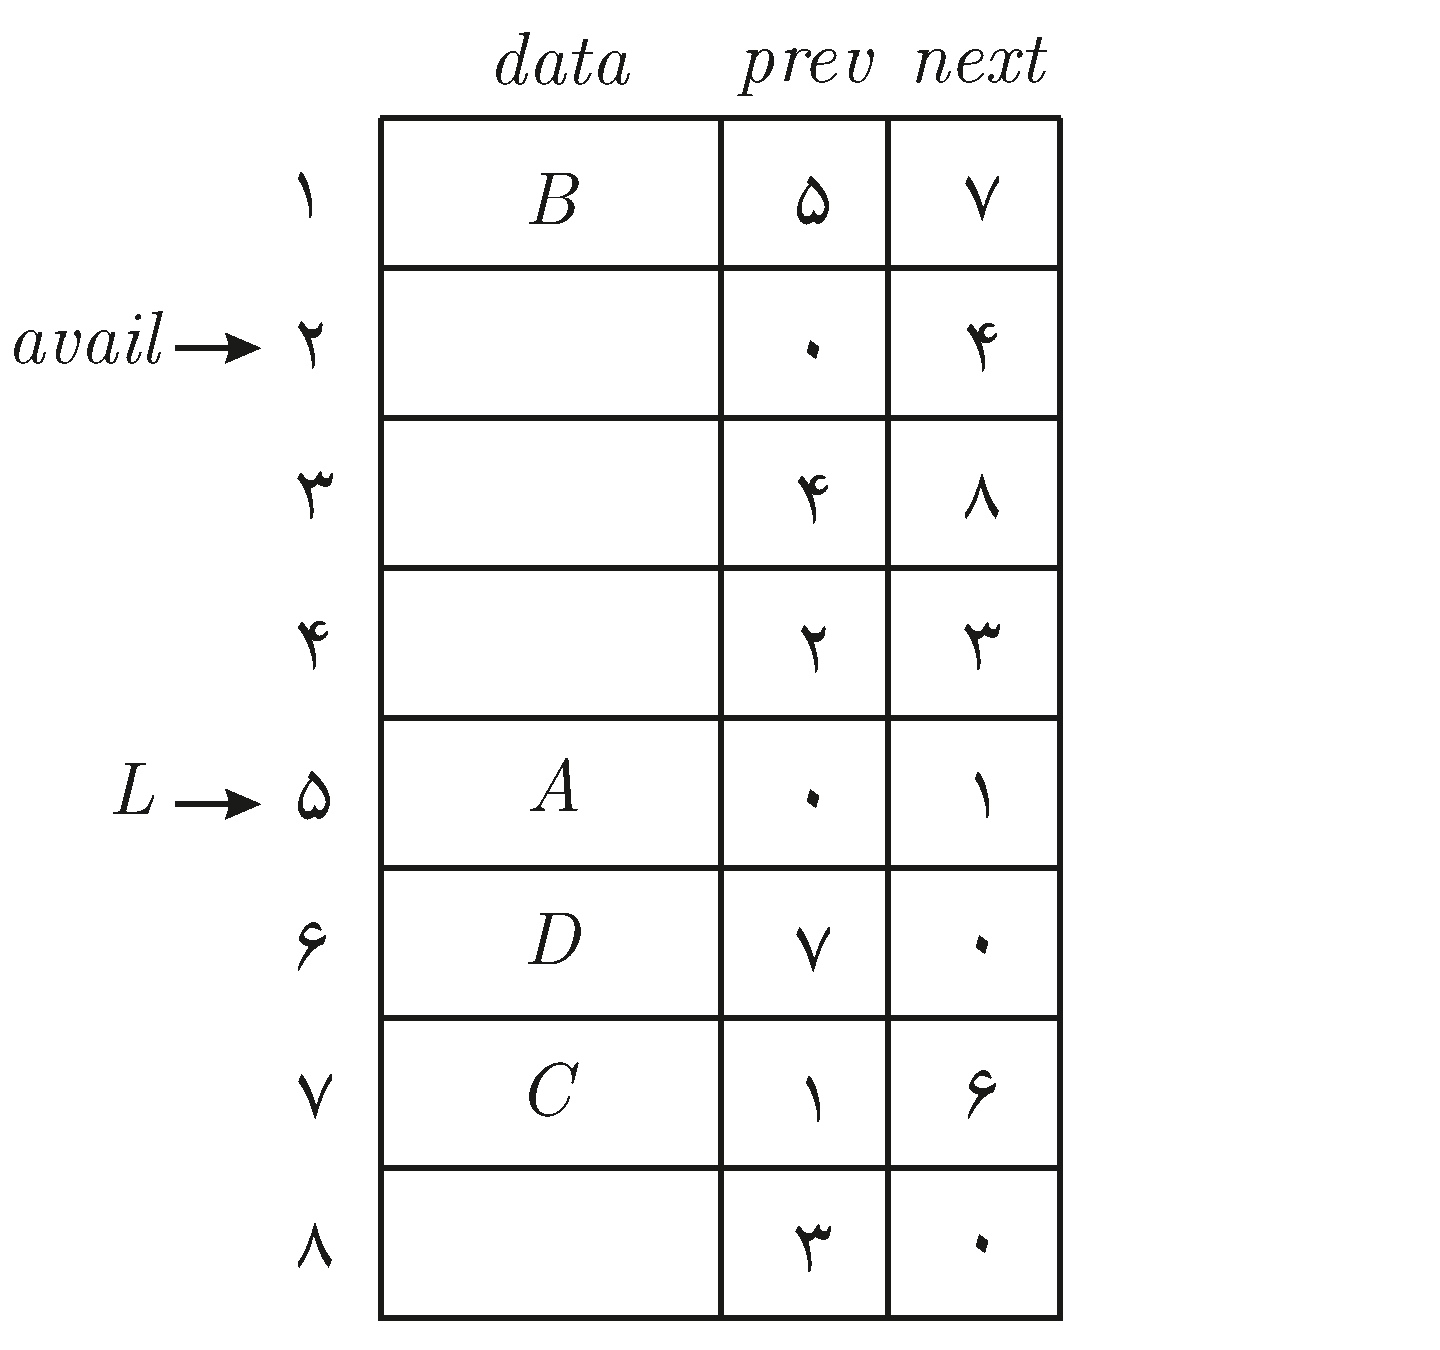
\includegraphics[scale=0.28]{figs/ch3/index_list_before_defrag.pdf}\label{ch3:fig:dblIdxLstBfrDefrag}
}
\subfloat[لیست اندیسی دوطرفه قسمت (آ) پس از یکپارچه‌سازی]{%
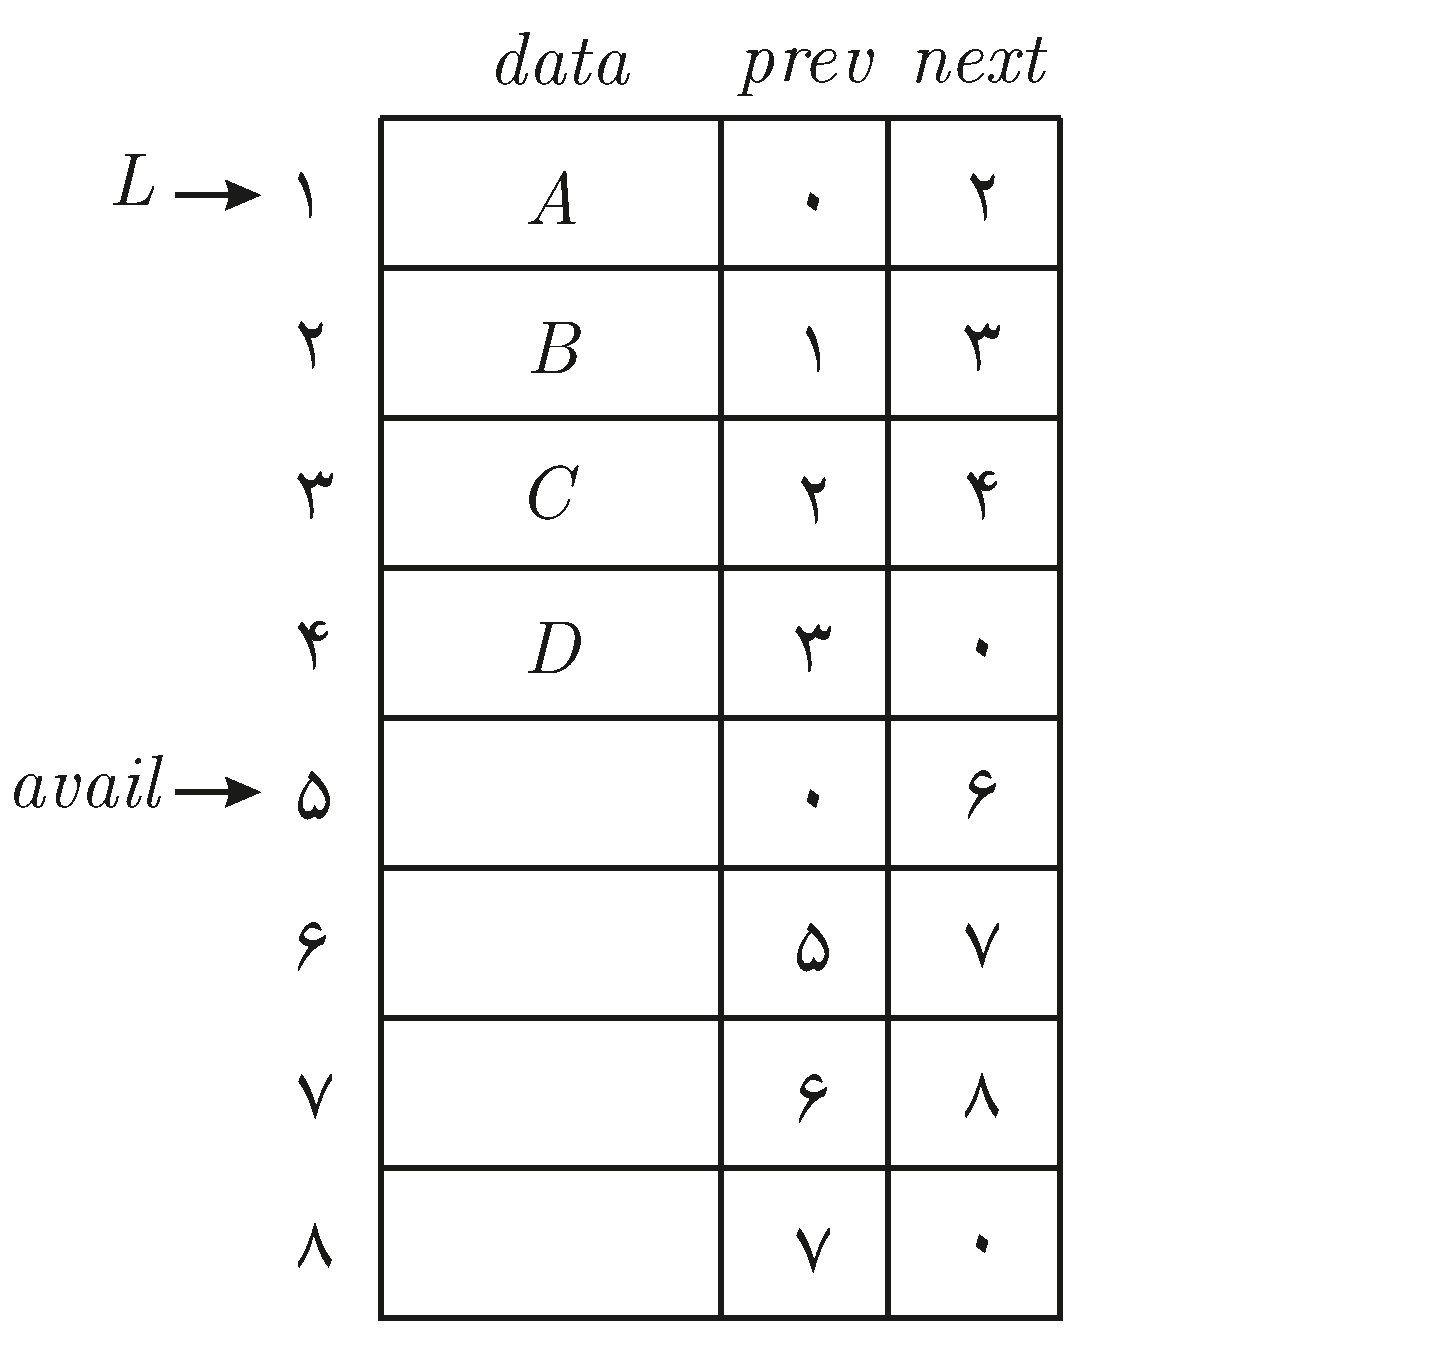
\includegraphics[scale=0.28]{figs/ch3/index_list_after_defrag.pdf}\label{ch3:fig:dblIdxLstAfrDefrag}
}
\caption{یکپارچه‌سازی یک لیست اندیسی دوطرفه}\label{ch3:fig:dblIdxLst}
\end{center}
\end{figure}

\سوال لیست اندیسی یکطرفه {$L$} را در نظر بگیرید که از آرایه‌ای به نام {\id{space}} برای ذخیره‌سازی عناصر استفاده می‌کند. زیربرنامه‌ای به نام {\bcall{Init}{}} بنویسید که خانه‌های آرایه‌ی {\id{space}} را طوری مقداردهی کند که آرایه آماده‌ی استفاده برای ذخیره‌سازی عناصر لیست شود.

\پاسخ

الگوریتم {\eqref{ch3:alg:initIdxLst}} نشان‌دهنده‌ی شبه کد آماده‌سازی یک لیست اندیسی یکطرفه برای ذخیره عناصر است. در این شبه کد فرض شده است طول آرایه {\id{space}} برابر با {\id{MAX}} است و همچنین {\id{avail}} نام اشاره‌گری است که باید به ابتدای لیست خانه‌های خالی آرایه اشاره کند.

روش کار الگوریتم {\eqref{ch3:alg:initIdxLst}} بسیار ساده است. در گام اول مقدار اشاره‌گر {\id{avail}} برابر با ۱ قرار داده می‌شود تا این اشاره‌گر به خانه اول آرایه اشاره کند. در گام دوم با استفاده از یک حلقه مقدار اشاره‌گر {\id{next}} هر خانه (به جز خانه آخر) از آرایه‌ی {\id{space}} برابر با شماره اندیس خانه بعدی آرایه قرار داده می‌شود. در گام آخر مقدار اشاره‌گر {\id{next}} خانه آخر و همچنین اشاره‌گر {$L$} برابر با صفر (که به معنی ثابت {\const{null}} است) قرار داده می‌شوند.

\begin{algorithm}
\caption{آماده‌سازی یک لیست اندیسی یکطرفه برای ذخیره‌سازی عناصر}\label{ch3:alg:initIdxLst}
\begin{latin}
\begin{algorithmic}[1]
\Procedure{Init}{$L$}
    \State    $\id{avail} \gets 1$
    \For{$i \gets 1 \To (\id{MAX} - 1)$}
        \State    $\attrib{space[i]}{next} \gets i + 1$
    \EndFor
    \State    $\attrib{space[MAX]}{next} \gets 0$
    \State    $L \gets 0$
\EndProcedure
\end{algorithmic}
\end{latin}
\end{algorithm}

\سوال دانشگاهی با ۴۰۰۰ دانشجو و ۲۰۰ درس را در نظر بگیرید. این دانشگاه برای سیستم آموزشی خود قصد تولید دو نوع گزارش را دارد:
\شروع{شمارش}
\فقره گزارشی شامل دانشجویان ثبت نام کننده در هر درس به تفکیک درس،
\فقره گزارشی شامل دروس ثبت نام شده توسط هر دانشجو به تفکیک دانشجو.
\پایان{شمارش}
یک راه برای ذخیره اطلاعات مربوط به دانشجویان و درس‌ها استفاده از یک آرایه دو بعدی است. چنین آرایه‌ای دارای ۸۰۰ هزار خانه خواهد بود! در این دانشگاه هر دانشجو به طور متوسط در سه درس ثبت نام می‌کند و این یعنی به طور متوسط تنها دوازده هزار خانه از این آرایه دارای مقادیر مفید هستند که برابر با {$1.5$} درصد از کل فضای آرایه است. در چنین حالتی فضای بسیار زیادی هدر می‌رود. به کمک لیست‌های پیوندی داده‌ساختاری طراحی کنید که فقط شامل اطلاعات مفید باشد و همچنین مناسب تولید دو نوع گزارش ذکر شده نیز باشد.

\پاسخ

شکل {\eqref{ch3:fig:customDS}} نمایش دهنده‌ی داده‌ساختار مورد نظر است. توجه داشته باشید که این داده‌ساختار تنها داده‌ساختار ممکن نیست. همانطور که از شکل مشخص است، چندین لیست پیوندی با یکدیگر ترکیب و در قالب یک لیست پیوندی پیچیده به نمایش درآمده‌اند. تمام لیست‌ها دارای گره‌ی سرلیست هستند و به صورت حلقوی پیاده‌سازی شده‌اند. روش به دست آوردن گزارش‌های ذکر شده در صورت سوال در ادامه بیان شده است.

\begin{figure}
\begin{center}
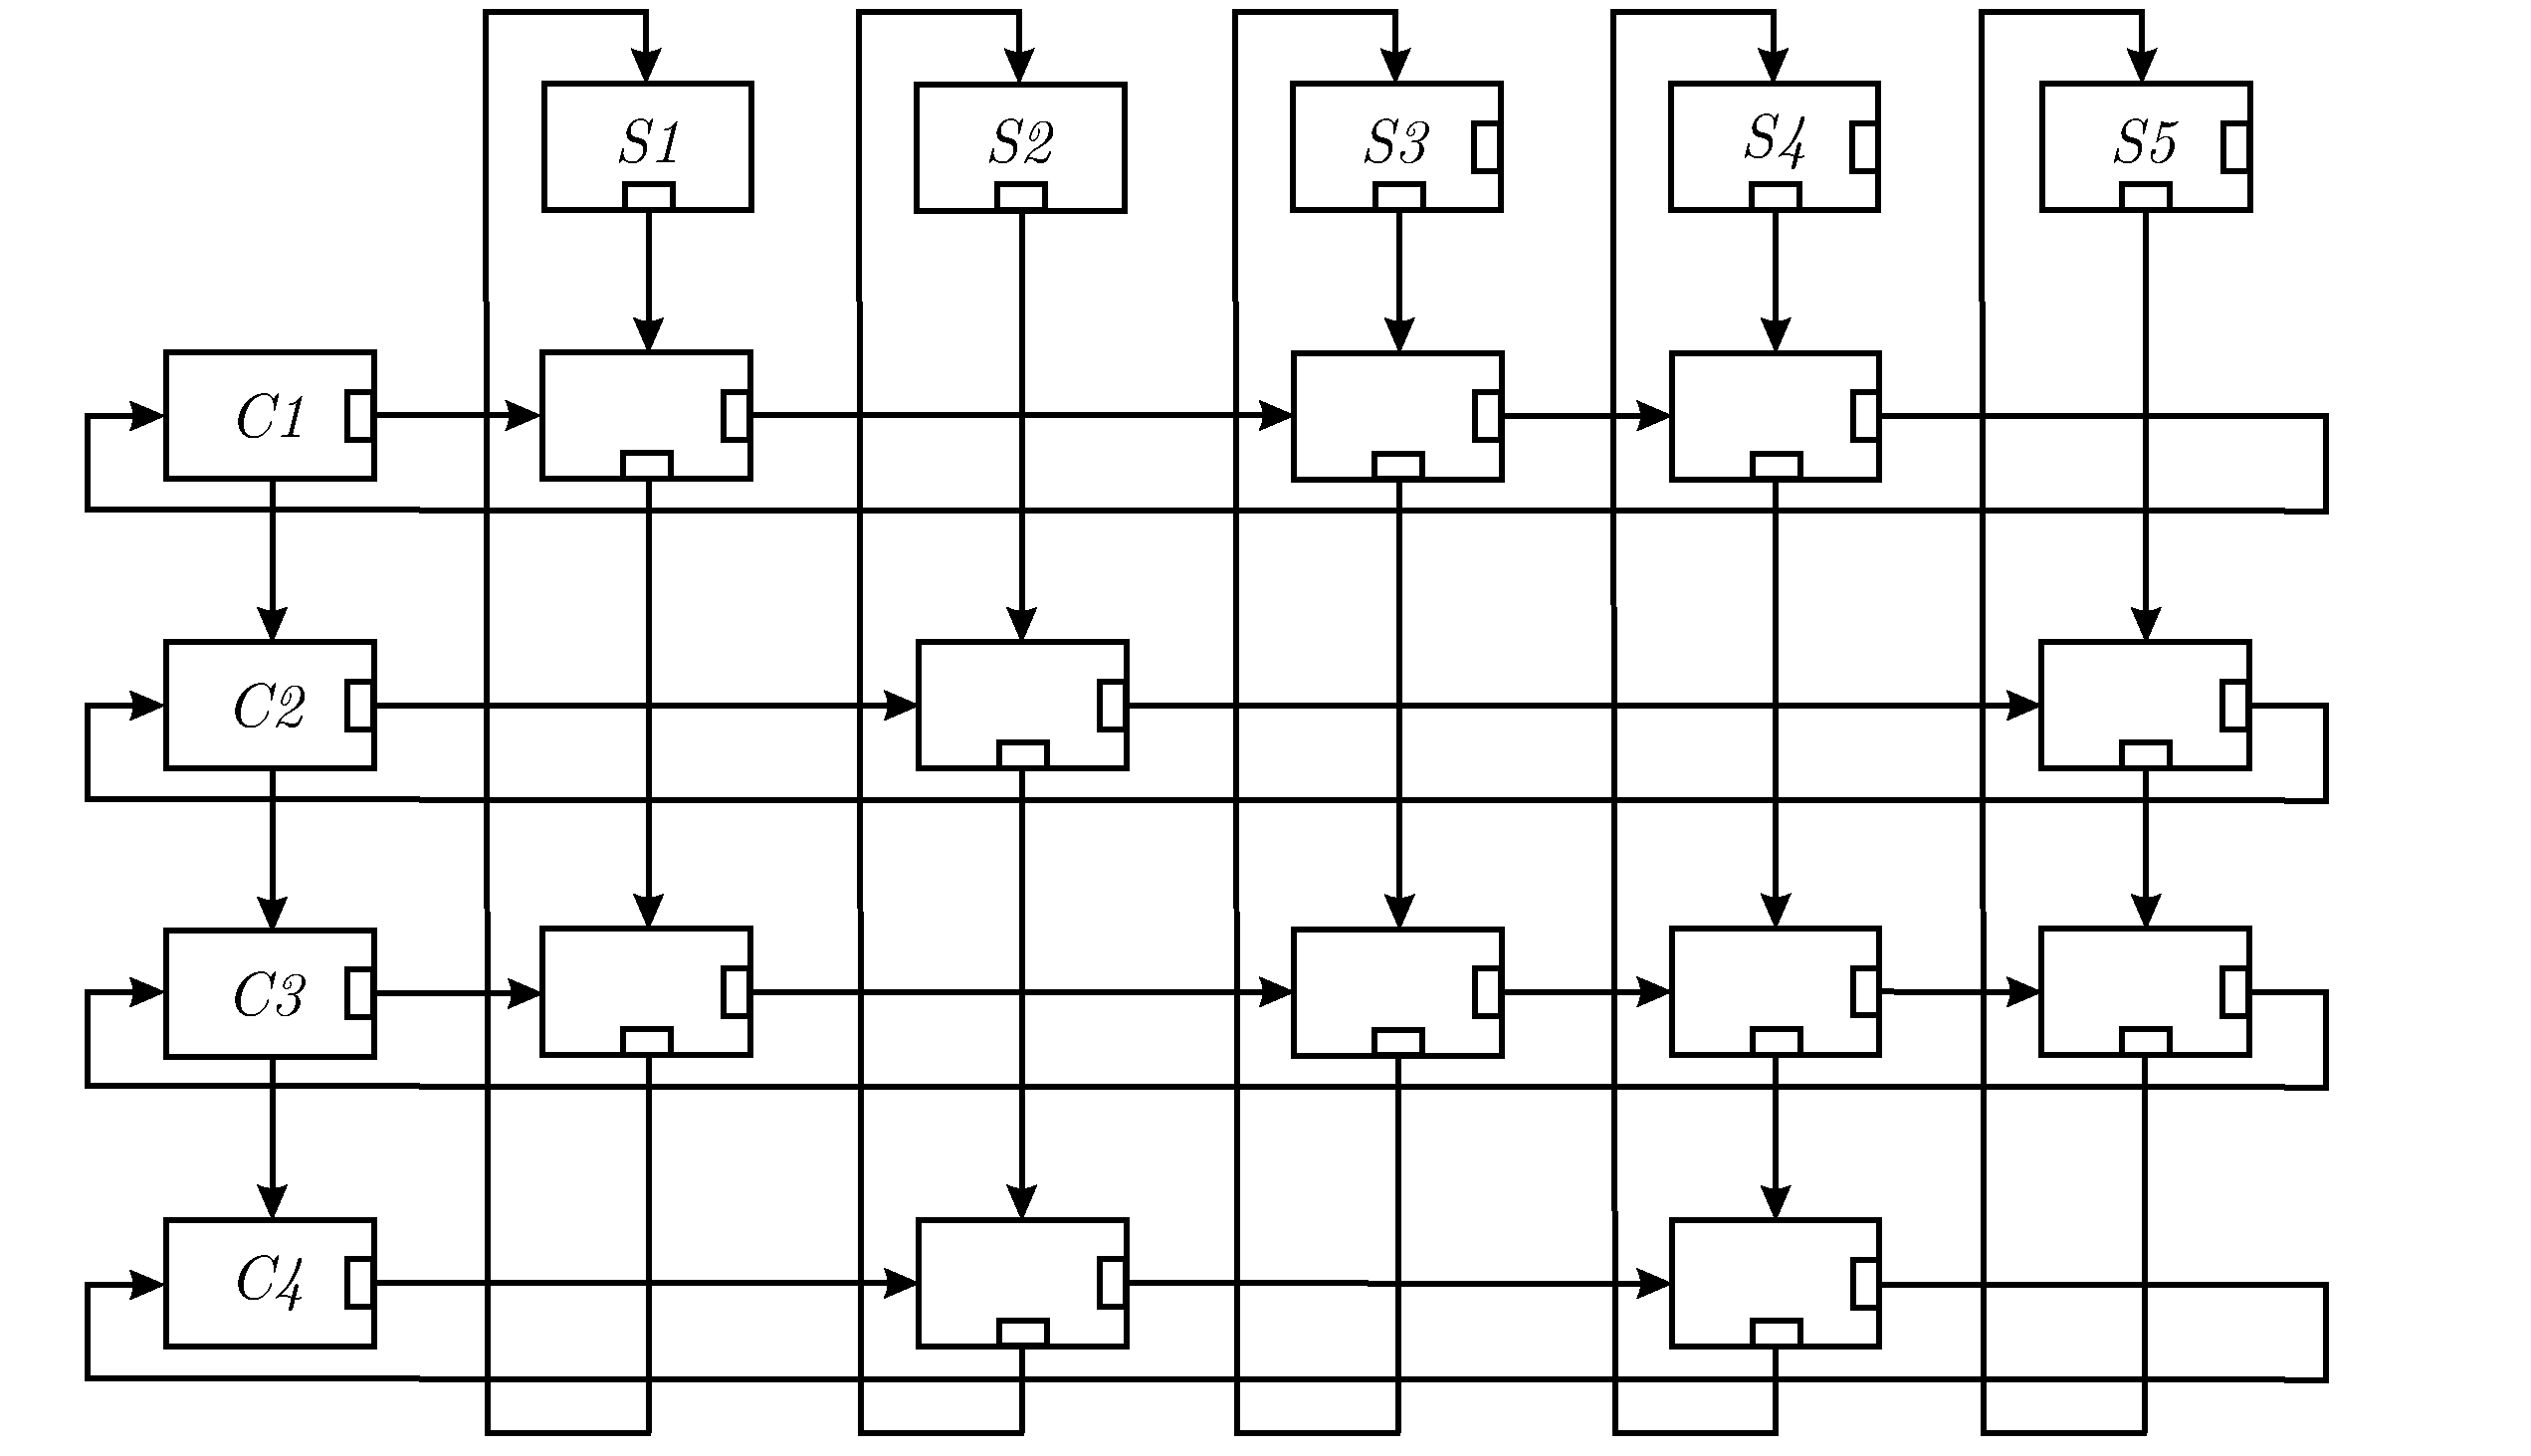
\includegraphics[scale=0.33]{figs/ch3/custom_ds.pdf}
\caption{%
یک داده‌ساختار مناسب برای گزارش‌گیری در مورد ۱) دانشجویان ثبت نام کننده در هر درس به تفکیک درس و ۲) دروس ثبت نام شده توسط هر دانشجو به تفکیک دانشجو.
}\label{ch3:fig:customDS}
\end{center}
\end{figure}

برای استخراج اسامی افراد ثبت‌نام کننده در یک درس، مثلاً درس {\lr{C3}} ، کافیست از گره با سرلیست {\lr{C3}} شروع کرده و به سمت راست این لیست حرکت کنیم. بعد از رفتن به اولین گره از لیست {\lr{C3}} ، مقدار جاری اشاره‌گر را ذخیره می‌کنیم و سپس با استفاده از اشاره‌گر به سمتِ پایین این گره، به صورت عمودی در لیست حرکت کرده تا به سرلیست لیست عمودی برسیم (در اینجا لیست {\lr{S1}}). به این ترتیب نام اولین دانشجو ثبت نام کننده در درس {\lr{C3}} به دست می‌‌آید. در گام بعد و برای به دست آوردن نام دانشجوی بعدی از اشاره‌گر ذخیره شده در گام قبل استفاده کرده و دوباره به سمت راست در لیست {\lr{C3}} حرکت کرده و روند حرکت عمودی در داده‌ساختار را ادامه می‌دهیم. به این ترتیب می‌توان اسامی تمام افراد ثبت نام کننده در یک درس را به دست آورد.

برای به دست آوردن دروس ثبت نام شده توسط یک دانشجو به روشی مشابه با پاراگراف قبل عمل می‌کنیم با این تفاوت که در اینجا از گره با سر لیست حاوی نام دانشجو شروع کرده و به سمت پایین لیست حرکت می‌کنیم و برای یافتن هر درس به صورت افقی لیست‌ها را پیمایش می‌کنیم.